% Options for packages loaded elsewhere
\PassOptionsToPackage{unicode}{hyperref}
\PassOptionsToPackage{hyphens}{url}
\PassOptionsToPackage{dvipsnames,svgnames*,x11names*}{xcolor}
%
\documentclass[
  11pt,
]{krantz}
\usepackage{amsmath,amssymb}
\usepackage{lmodern}
\usepackage{ifxetex,ifluatex}
\ifnum 0\ifxetex 1\fi\ifluatex 1\fi=0 % if pdftex
  \usepackage[T1]{fontenc}
  \usepackage[utf8]{inputenc}
  \usepackage{textcomp} % provide euro and other symbols
\else % if luatex or xetex
  \usepackage{unicode-math}
  \defaultfontfeatures{Scale=MatchLowercase}
  \defaultfontfeatures[\rmfamily]{Ligatures=TeX,Scale=1}
  \setmonofont[Scale=0.7]{Source Code Pro}
\fi
% Use upquote if available, for straight quotes in verbatim environments
\IfFileExists{upquote.sty}{\usepackage{upquote}}{}
\IfFileExists{microtype.sty}{% use microtype if available
  \usepackage[]{microtype}
  \UseMicrotypeSet[protrusion]{basicmath} % disable protrusion for tt fonts
}{}
\makeatletter
\@ifundefined{KOMAClassName}{% if non-KOMA class
  \IfFileExists{parskip.sty}{%
    \usepackage{parskip}
  }{% else
    \setlength{\parindent}{0pt}
    \setlength{\parskip}{6pt plus 2pt minus 1pt}}
}{% if KOMA class
  \KOMAoptions{parskip=half}}
\makeatother
\usepackage{xcolor}
\IfFileExists{xurl.sty}{\usepackage{xurl}}{} % add URL line breaks if available
\IfFileExists{bookmark.sty}{\usepackage{bookmark}}{\usepackage{hyperref}}
\hypersetup{
  pdftitle={Elementos de la estadística},
  pdfauthor={Ricardo Michel MALLQUI BAÑOS},
  colorlinks=true,
  linkcolor=Maroon,
  filecolor=Maroon,
  citecolor=Blue,
  urlcolor=Blue,
  pdfcreator={LaTeX via pandoc}}
\urlstyle{same} % disable monospaced font for URLs
\usepackage{color}
\usepackage{fancyvrb}
\newcommand{\VerbBar}{|}
\newcommand{\VERB}{\Verb[commandchars=\\\{\}]}
\DefineVerbatimEnvironment{Highlighting}{Verbatim}{commandchars=\\\{\}}
% Add ',fontsize=\small' for more characters per line
\usepackage{framed}
\definecolor{shadecolor}{RGB}{248,248,248}
\newenvironment{Shaded}{\begin{snugshade}}{\end{snugshade}}
\newcommand{\AlertTok}[1]{\textcolor[rgb]{0.94,0.16,0.16}{#1}}
\newcommand{\AnnotationTok}[1]{\textcolor[rgb]{0.56,0.35,0.01}{\textbf{\textit{#1}}}}
\newcommand{\AttributeTok}[1]{\textcolor[rgb]{0.77,0.63,0.00}{#1}}
\newcommand{\BaseNTok}[1]{\textcolor[rgb]{0.00,0.00,0.81}{#1}}
\newcommand{\BuiltInTok}[1]{#1}
\newcommand{\CharTok}[1]{\textcolor[rgb]{0.31,0.60,0.02}{#1}}
\newcommand{\CommentTok}[1]{\textcolor[rgb]{0.56,0.35,0.01}{\textit{#1}}}
\newcommand{\CommentVarTok}[1]{\textcolor[rgb]{0.56,0.35,0.01}{\textbf{\textit{#1}}}}
\newcommand{\ConstantTok}[1]{\textcolor[rgb]{0.00,0.00,0.00}{#1}}
\newcommand{\ControlFlowTok}[1]{\textcolor[rgb]{0.13,0.29,0.53}{\textbf{#1}}}
\newcommand{\DataTypeTok}[1]{\textcolor[rgb]{0.13,0.29,0.53}{#1}}
\newcommand{\DecValTok}[1]{\textcolor[rgb]{0.00,0.00,0.81}{#1}}
\newcommand{\DocumentationTok}[1]{\textcolor[rgb]{0.56,0.35,0.01}{\textbf{\textit{#1}}}}
\newcommand{\ErrorTok}[1]{\textcolor[rgb]{0.64,0.00,0.00}{\textbf{#1}}}
\newcommand{\ExtensionTok}[1]{#1}
\newcommand{\FloatTok}[1]{\textcolor[rgb]{0.00,0.00,0.81}{#1}}
\newcommand{\FunctionTok}[1]{\textcolor[rgb]{0.00,0.00,0.00}{#1}}
\newcommand{\ImportTok}[1]{#1}
\newcommand{\InformationTok}[1]{\textcolor[rgb]{0.56,0.35,0.01}{\textbf{\textit{#1}}}}
\newcommand{\KeywordTok}[1]{\textcolor[rgb]{0.13,0.29,0.53}{\textbf{#1}}}
\newcommand{\NormalTok}[1]{#1}
\newcommand{\OperatorTok}[1]{\textcolor[rgb]{0.81,0.36,0.00}{\textbf{#1}}}
\newcommand{\OtherTok}[1]{\textcolor[rgb]{0.56,0.35,0.01}{#1}}
\newcommand{\PreprocessorTok}[1]{\textcolor[rgb]{0.56,0.35,0.01}{\textit{#1}}}
\newcommand{\RegionMarkerTok}[1]{#1}
\newcommand{\SpecialCharTok}[1]{\textcolor[rgb]{0.00,0.00,0.00}{#1}}
\newcommand{\SpecialStringTok}[1]{\textcolor[rgb]{0.31,0.60,0.02}{#1}}
\newcommand{\StringTok}[1]{\textcolor[rgb]{0.31,0.60,0.02}{#1}}
\newcommand{\VariableTok}[1]{\textcolor[rgb]{0.00,0.00,0.00}{#1}}
\newcommand{\VerbatimStringTok}[1]{\textcolor[rgb]{0.31,0.60,0.02}{#1}}
\newcommand{\WarningTok}[1]{\textcolor[rgb]{0.56,0.35,0.01}{\textbf{\textit{#1}}}}
\usepackage{longtable,booktabs,array}
\usepackage{calc} % for calculating minipage widths
% Correct order of tables after \paragraph or \subparagraph
\usepackage{etoolbox}
\makeatletter
\patchcmd\longtable{\par}{\if@noskipsec\mbox{}\fi\par}{}{}
\makeatother
% Allow footnotes in longtable head/foot
\IfFileExists{footnotehyper.sty}{\usepackage{footnotehyper}}{\usepackage{footnote}}
\makesavenoteenv{longtable}
\usepackage{graphicx}
\makeatletter
\def\maxwidth{\ifdim\Gin@nat@width>\linewidth\linewidth\else\Gin@nat@width\fi}
\def\maxheight{\ifdim\Gin@nat@height>\textheight\textheight\else\Gin@nat@height\fi}
\makeatother
% Scale images if necessary, so that they will not overflow the page
% margins by default, and it is still possible to overwrite the defaults
% using explicit options in \includegraphics[width, height, ...]{}
\setkeys{Gin}{width=\maxwidth,height=\maxheight,keepaspectratio}
% Set default figure placement to htbp
\makeatletter
\def\fps@figure{htbp}
\makeatother
\setlength{\emergencystretch}{3em} % prevent overfull lines
\providecommand{\tightlist}{%
  \setlength{\itemsep}{0pt}\setlength{\parskip}{0pt}}
\setcounter{secnumdepth}{5}
\usepackage[spanish,es-lcroman,es-tabla]{babel}
\usepackage{booktabs}
\usepackage{graphicx}
\usepackage{amsmath}
\usepackage{makeidx}
\usepackage{array}% http://ctan.org/pkg/array
\makeindex


\usepackage{enumitem}
\setlist[enumerate]{leftmargin=10mm, label=\alph*)}
\setlist[itemize]{leftmargin=10mm}


\makeatletter\@addtoreset{chapter}{part}\makeatother%

%\usepackage{showframe}
%\usepackage[a4paper]{geometry}
%\geometry{verbose,tmargin=3cm,bmargin=3cm,lmargin=3.5cm,rmargin=3cm}
\setlength{\tabcolsep}{0.38em}
%\renewcommand{\arraystretch}{1.5}

\usepackage{times}
\renewcommand{\rmdefault}{ptm}
%\usepackage[lite,subscriptcorrection,nofontinfo,zswash]{mtpro2}

\usepackage{graphicx}

% Determine if the image is too wide for the page.
\makeatletter
\def\ScaleIfNeeded{%
  \ifdim\Gin@nat@width>\linewidth
    \linewidth
  \else
    \Gin@nat@width
  \fi
}
\makeatother

% Resize figures that are too wide for the page.
%\let\oldincludegraphics\includegraphics
%\renewcommand\includegraphics[2][]{%
%  \oldincludegraphics[scale=0.85]{#2}
%}

\usepackage{amsthm}
\makeatletter
\def\thm@space@setup{%
  \thm@preskip=8pt plus 2pt minus 4pt
  \thm@postskip=\thm@preskip
}
\makeatother



%\flushbottom

\frontmatter
\ifluatex
  \usepackage{selnolig}  % disable illegal ligatures
\fi
\usepackage[]{natbib}
\bibliographystyle{apalike}

\title{Elementos de la estadística}
\usepackage{etoolbox}
\makeatletter
\providecommand{\subtitle}[1]{% add subtitle to \maketitle
  \apptocmd{\@title}{\par {\large #1 \par}}{}{}
}
\makeatother
\subtitle{estadística descriptiva y probabilidades}
\author{Ricardo Michel MALLQUI BAÑOS}
\date{2022-09-26}

\usepackage{amsthm}
\newtheorem{theorem}{Teorema}[chapter]
\newtheorem{lemma}{Lema}[chapter]
\newtheorem{corollary}{Corolario}[chapter]
\newtheorem{proposition}{Proposición}[chapter]
\newtheorem{conjecture}{Conjectura}[chapter]
\theoremstyle{definition}
\newtheorem{definition}{Definición}[chapter]
\theoremstyle{definition}
\newtheorem{example}{Ejemplo}[chapter]
\theoremstyle{definition}
\newtheorem{exercise}{Ejercicio}[chapter]
\theoremstyle{definition}
\newtheorem{hypothesis}{Hypothesis}[chapter]
\theoremstyle{remark}
\newtheorem*{remark}{Observación}
\newtheorem*{solution}{Solución}
\begin{document}
\maketitle

%\cleardoublepage\newpage\thispagestyle{empty}\null
%\cleardoublepage\newpage\thispagestyle{empty}\null
%\cleardoublepage\newpage
\thispagestyle{empty}
\begin{center}

\includegraphics{U.pdf}
\end{center}

%\setlength{\abovedisplayskip}{-5pt}
%\setlength{\abovedisplayshortskip}{-5pt}

{
\hypersetup{linkcolor=}
\setcounter{tocdepth}{2}
\tableofcontents
}
\listoftables
\listoffigures
\newcommand{\N}{\mathbb{N}}
\newcommand{\R}{\mathbb{R}}
\newcommand{\CC}{\mathbb{C}}
\newcommand{\I}{\mathbb{I}}
\newcommand{\f}{\mathbb{f}}
\newcommand{\X}{\mathbb{X}}
\newcommand{\D}{\mathbb{D}}
\newcommand{\Z}{\mathbb{Z}}
\newcommand{\Q}{\mathbb{Q}}
\newcommand{\norm}[1]{\left\Vert#1\right\Vert}
\newcommand{\abs}[1]{\left\vert#1\right\vert}
\newcommand{\set}[1]{\left\{#1\right\}}
\newcommand{\seq}[1]{\left<#1\right>}
\newcommand{\co}[1]{\left[#1\right]}
\newcommand{\cc}[1]{\left(#1\right)}
\newcommand{\J}{\mathcal{J}}
\newcommand{\K}{\mathcal{K}}
\newcommand{\M}{\mathcal{M}}
\newcommand{\F}{\mathcal{F}}

\hypertarget{resumen}{%
\chapter*{Resumen}\label{resumen}}


La estadística es la ciencia que manipula datos las analiza e interpreta para poder sacar concluciones razonables de ciertos fenomenos naturales. Esta ciencia puede ser dividido en dos: \textbf{estadística descirptiva} y \textbf{estadística inferencial}. En la estadística descriptiva se procesan datos de una manera teórica y utilitaria. Estos métodos consisten en la recolección, organización, resumen, descripcion y presenatacion de la información. Si la poblacion está disponible entonces la estadística descriptiva es suficiente para describir ciertos fenomenos. No obstante generalmente no se dispone de toda la población si no de una muestra de ella, es en este caso que se requieren usar técnicas más sofisticadas para tomar decisiones y generalizaciones acerca de la poblacion, desde una pequeña muestra de información. Es cuando entra en el juego la estadística inferencial.

La base teórica de la estadística son las matemáticas

Este libro se compone de dos partes, la primera parte trata sobre la \textbf{estadística descirptiva} y la segunda \textbf{estadística inferencial}. Cada una de ellas divididas en capítulos.

\mainmatter

\hypertarget{part-estaduxedstica-descriptiva}{%
\part{Estadística descriptiva}\label{part-estaduxedstica-descriptiva}}

\hypertarget{preliminares}{%
\chapter{Preliminares}\label{preliminares}}

\hypertarget{pre-requisitos}{%
\section{Pre requisitos}\label{pre-requisitos}}

Estar familiarizado con las nociones de matemáticas básicas, \textbf{cálculo diferencial e integral}.

\hypertarget{definiciones-buxe1sicas}{%
\section{Definiciones básicas}\label{definiciones-buxe1sicas}}

\begin{definition}[Estadística]
\protect\hypertarget{def:std}{}\label{def:std}Es la ciencia de los datos. Es decir colecciona, clasifica, resume, organiza, analiza e interpreta datos
\end{definition}

La estadística es comúnmente aplicada a dos tipos de problemas:

\begin{enumerate}
\def\labelenumi{\arabic{enumi}.}
\tightlist
\item
  Resumiendo, describiendo y explorando datos.
\item
  Usando muestra de datos para inferir la naturaleza de un conjunto de datos del cual se extrajo la muestra seleccionada.
\end{enumerate}

\begin{definition}[Estadística descriptiva]
\protect\hypertarget{def:descriptiva}{}\label{def:descriptiva}The branch of statistics devoted to the organization, summarization, and description of data sets is
called descriptive statistics.
\end{definition}

\begin{definition}[Estadística inferencial]
\protect\hypertarget{def:inferencial}{}\label{def:inferencial}The branch of statistics concerned with using sample data to make an inference about a large set of
data is called inferential statistics.
\end{definition}

\begin{definition}[Muestra]
\protect\hypertarget{def:muestra}{}\label{def:muestra}A sample is a subset of data selected from the target population.
\end{definition}

\begin{definition}[Unidad]
\protect\hypertarget{def:unidad}{}\label{def:unidad}The object (e.g., person, thing, transaction, specimen, or event) upon which measurements are
collected is called the experimental unit. (Note: A population consists of data collected on many
experimental units.)
\end{definition}

\hypertarget{elementos-fundamentales-de-la-estaduxedstica}{%
\section{Elementos fundamentales de la estadística}\label{elementos-fundamentales-de-la-estaduxedstica}}

\begin{definition}[Poblacion]
\protect\hypertarget{def:poblacion}{}\label{def:poblacion}A statistical population is a data set (usually large, sometimes conceptual) that is our target of interest.
\end{definition}

\begin{definition}[Variables cuantitativas]
\protect\hypertarget{def:variable2}{}\label{def:variable2}

Una variable estadística es una \textbf{característica} que puede fluctuar y cuya \textbf{variación} es susceptible de adoptar \textbf{diferentes valores}, los cuales pueden medirse u observarse. Las variables adquieren valor cuando se relacionan con otras variables, es decir, si forman parte de una \textbf{hipótesis} o de una \textbf{teoría}. Existen dos clases de variables: Cualitativas y cuantitativas.

\begin{enumerate}
\def\labelenumi{\arabic{enumi}.}
\item
  \textbf{Cualitativas}. Son aquellas variables que están propensos a ser nominadas textualmente.

  \begin{itemize}
  \item
    \textbf{Nominales}. Son características que simplemente nominan y están propensos a ser jerarquizados u ordenados tales como: El estado civil (soltero, casado, divorciado, viudo), Religión (católica, evangélico, judío, etc).
  \item
    \textbf{Ordinales}. Son características que que si están propensos a ser jerarquizados tales como: Nivel de instrucción (inicial, primaria, secundaria, superior).
  \end{itemize}
\item
  \textbf{cuantitativas}. Son aquellas variables que están propensos a ser medidas mediante números ya sean números enteros o reales.

  \begin{itemize}
  \item
    \textbf{Discretas}. Aquellas que solo son medidos mediante números enteros por ejemplo: Número de hijos, número de habitaciones.
  \item
    \textbf{Continuas}. Aquellas que solo son medidos mediante números reales es decir este incluye a los números racionales e irracionales. Estatura, volumen, peso.
  \end{itemize}
\end{enumerate}

\end{definition}

\hypertarget{organizaciuxf3n-de-datos-en-tablas-de-frecuencias}{%
\chapter{Organización de datos en tablas de frecuencias}\label{organizaciuxf3n-de-datos-en-tablas-de-frecuencias}}

\hypertarget{distribuciuxf3n-de-frecuencias}{%
\section{Distribución de frecuencias}\label{distribuciuxf3n-de-frecuencias}}

El uso de tablas de distribución de frecuencias y gráficas como un medio para presentar la información
de un conjunto de datos de forma resumida. En grados anteriores ya se ha trabajado con gráficas para
variables cuantitativas discretas, por lo que esta será la primera vez que el estudiante trabajará con
gráficas que son adecuadas para presentar información de variables cuantitativas continuas.

\begin{definition}
La tabulación es un proceso en el cual los datos son ordenados en grupos llamados \emph{clases} para un análisis más eficaz de estos, los datos podrían estar clasificados mediante una variable cualitativa o cuantitativa en el caso de las variables cualitativas \(Y_i\), se considera la siguiente Tabla \ref{tab:ww}
\end{definition}

\begin{longtable}[]{@{}cccccccccc@{}}
\caption{\label{tab:ww} Caption}\tabularnewline
\toprule
\(Y_i\) & \(f_i\) & \(F_i\) & \(F_i^*\) & \(h_i\) & \(H_i\) & \(H_i^*\) & \(h_i\%\) & \(H_i\%\) & \(H_i^*\%\) \\
\midrule
\endfirsthead
\toprule
\(Y_i\) & \(f_i\) & \(F_i\) & \(F_i^*\) & \(h_i\) & \(H_i\) & \(H_i^*\) & \(h_i\%\) & \(H_i\%\) & \(H_i^*\%\) \\
\midrule
\endhead
\(Y_1\) & \(f_1\) & \(F_1\) & \(F_1^*\) & \(\frac{f_1}{n}\) & \(\frac{F_1}{n}\) & \(\frac{F_1^*}{n}\) & \(h_1\) & \(H_1\) & \(H_1^*\) \\
\(Y_2\) & \(f_2\) & \(F_2\) & \(F_2^*\) & \(\frac{f_2}{n}\) & \(\frac{F_2}{n}\) & \(\frac{F_2^*}{n}\) & \(h_2\) & \(H_2\) & \(H_1^*\) \\
\(Y_3\) & \(f_3\) & \(F_3\) & \(F_3^*\) & \(\frac{f_3}{n}\) & \(\frac{F_3}{n}\) & \(\frac{F_3^*}{n}\) & \(h_3\) & \(H_3\) & \(H_1^*\) \\
\(\vdots\) & \(\vdots\) & \(\vdots\) & \(\vdots\) & \(\vdots\) & \(\vdots\) & \(\vdots\) & \(\vdots\) & \(\vdots\) & \(\vdots\) \\
\(Y_r\) & \(f_r\) & \(F_r\) & \(F_r^*\) & \(\frac{f_r}{n}\) & \(\frac{F_r}{n}\) & \(\frac{F_r^*}{n}\) & \(h_r\) & \(H_r\) & \(H_1^*\) \\
\bottomrule
\end{longtable}

En el caso de variables cuantitativas ademas si los datos son muy variados, que para se clasificados adecuadamente, necesitan generarse particiones de longitudes semejantes entonces se utiliza el siguiente proceso; el \textbf{número de las particiones} \(r\) se consideran de acuerdo a \textbf{tres criterios}.

\begin{enumerate}
\def\labelenumi{\arabic{enumi}.}
\tightlist
\item
  Criterio del investigador \(r\) no puede ser más de 20 ni menos de 5
\item
  \(r=\sqrt{n}\) donde \(n\) es el número de datos
\item
  La regla de Starges que consiste en considerar la fórmula \(r=3.322\cdot\log_{10} n\) Una vez establecido el número de particiones se procede a generar los límites laterales de cada una de las particiones, sea \(L\) la longitud de todo el conjunto es decir \(L=x_{\text{max}}-x_{\text{min}}\) entonces la longitud de las particiones o amplitud interválica se obtiene con \(l=\frac{L}{r}\)
\end{enumerate}

\begin{longtable}[t]{ccccccccccc}
\caption{\label{tab:cuantitativaw}Datos cuantitativos (intervalos)}\\
\toprule
Clase & $Y_i$ & $f_i$ & $F_i$ & $F_i^*$ & $h_i$ & $H_i$ & $H_i^*$ & $h_i\%$ & $H_i\%$ & $H_i^*\%$\\
\midrule
$[y_1-y_2)$ & $Y_1$ & $f_i$ & $F_i$ & $F_i^*$ & $\frac{f_1}{n}$ & $\frac{f_1}{n}$ & $\frac{F_1^*}{n}$ & $h_1\%$ & $H_1\%$ & $H_1^*\%$\\
$[y_2-y_3)$ & $Y_2$ & $f_i$ & $F_i$ & $F_i^*$ & $\frac{f_2}{n}$ & $\frac{f_1}{n}$ & $\frac{F_1^*}{n}$ & $h_2\%$ & $H_2\%$ & $H_2^*\%$\\
$\ldots$ & $\ldots$ & $\ldots$ & $\ldots$ & $\ldots$ & $\ldots$ & $\ldots$ & $\ldots$ & $\ldots$ & $\ldots$ & $\ldots$\\
$[y_{r-1}-y_r)$ & $Y_r$ & $f_r$ & $F_r$ & $F_r^*$ & $\frac{f_r}{n}$ & $\frac{f_1}{n}$ & $\frac{F_r^*}{n}$ & $h_r\%$ & $H_r\%$ & $H_r^*\%$\\
\bottomrule
\end{longtable}

Tenga en cuenta que \(n\) es el número de datos, es decir \(n=f_1+f_2+\ldots+f_r=\sum_{i=1}^r\) donde \(f_i\) es número de datos en la partición \(X_i\), una de las \(r\) particiones del conjunto total de datos.

\begin{enumerate}
\def\labelenumi{\arabic{enumi}.}
\item
  Las \textbf{frecuencias absolutas}\index{frecuencias absolutas} \(f_i\) indican el número de datos con la característica \(X_i\).
\item
  Las \textbf{frecuencias absolutas acumuladas menor que}\index{frecuencias absolutas acumuladas menor que} \(F_i\) obedecen a la fórmula \[F_m=f_1+f_2+\ldots+f_m=\sum_{i=1}^mf_i\]
\item
  Las \textbf{frecuencias absolutas acumuladas mayor que} \(F_i^*\) obedecen a la fórmula \[
  \begin{aligned}
  F_m^*&=f_m+f_{m+1}+\ldots+f_r\\
  &=\sum_{i=m}^rf_i\\
  &=n-\sum_{i=1}^{m-1}f_i\\
  &=n-\left(f_1+f_{2}+\ldots+f_{m-1}\right)
  \end{aligned}
  \]
\item
  Las \textbf{frecuencias absolutas relativas}\index{frecuencias absolutas relativas} obedecen a la fórmula \[h_m=\frac{f_m}{n}\]
\item
  Las \textbf{frecuencias absolutas relativas menor que}\index{frecuencias absolutas relativas  menor que} obedecen a la fórmula \[H_m=\frac{f_m}{n}\]
\item
  Las \textbf{frecuencias absolutas relativas mayor que} obedecen a la fórmula \[H_m^*=\frac{F_m}{n}\]
\item
  Las \textbf{frecuencias absolutas relativas porcentuales} obedecen a la fórmula \(h_i\%=100\cdot h_i\)
\item
  Las \textbf{frecuencias absolutas relativas menor que porcentuales} obedecen a la fórmula \(H_i\%=100\cdot H_i\)
\item
  Las \textbf{frecuencias absolutas relativas mayor que porcentuales} obedecen a la fórmula \(H_i^*\%=100\cdot H_i^*\)
\item
  \(Y_i\) marca de clase o punto medio de la clase \(i\)
\end{enumerate}

\begin{example}

Sean Los 16 tipos de personalidad en un grupo social encuestado. Organice los datos en una tabla de frecuencias

\begin{longtable}[t]{cccccccccc}
\caption{\label{tab:cualitativa}Datos cualitativos}\\
\toprule
$Y_i$ & $f_i$ & $F_i$ & $F_i^*$ & $h_i$ & $H_i$ & $H_i^*$ & $h_i\%$ & $H_i\%$ & $H_i^*\%$\\
\midrule
ESTJ & 1 & 1 & 75 & 0.01 & 0.01 & 1.00 & 1.33 & 1.33 & 100.00\\
ESTJ & 2 & 3 & 150 & 0.03 & 0.04 & 2.00 & 2.67 & 4.00 & 200.00\\
ESTP & 3 & 6 & 150 & 0.04 & 0.08 & 2.00 & 4.00 & 8.00 & 200.00\\
ESFJ & 4 & 10 & 150 & 0.05 & 0.13 & 2.00 & 5.33 & 13.33 & 200.00\\
ESFP & 6 & 16 & 150 & 0.08 & 0.21 & 2.00 & 8.00 & 21.33 & 200.00\\
ISTJ & 6 & 22 & 155 & 0.08 & 0.29 & 2.07 & 8.00 & 29.33 & 206.67\\
ISTP & 7 & 29 & 157 & 0.09 & 0.39 & 2.09 & 9.33 & 38.67 & 209.33\\
ISFJ & 8 & 37 & 158 & 0.11 & 0.49 & 2.11 & 10.67 & 49.33 & 210.67\\
ISFP & 9 & 46 & 166 & 0.12 & 0.61 & 2.21 & 12.00 & 61.33 & 221.33\\
ENTJ & 10 & 56 & 166 & 0.13 & 0.75 & 2.21 & 13.33 & 74.67 & 221.33\\
ENTP & 6 & 62 & 166 & 0.08 & 0.83 & 2.21 & 8.00 & 82.67 & 221.33\\
ENFJ & 5 & 67 & 166 & 0.07 & 0.89 & 2.21 & 6.67 & 89.33 & 221.33\\
ENFP & 3 & 70 & 166 & 0.04 & 0.93 & 2.21 & 4.00 & 93.33 & 221.33\\
INTJ & 2 & 72 & 167 & 0.03 & 0.96 & 2.23 & 2.67 & 96.00 & 222.67\\
INTP & 1 & 73 & 169 & 0.01 & 0.97 & 2.25 & 1.33 & 97.33 & 225.33\\
INFJ & 1 & 74 & 172 & 0.01 & 0.99 & 2.29 & 1.33 & 98.67 & 229.33\\
INFP & 1 & 75 & 176 & 0.01 & 1.00 & 2.35 & 1.33 & 100.00 & 234.67\\
TOTAL & 75 &  &  &  &  &  & 100.00 &  & \\
\bottomrule
\end{longtable}

\end{example}

\begin{example}

Edades de cierta comunidad

25
35 38
45 47 48
51 52 53 55
60 62 63 66 67
70 71 72 75 77 78
81 88 89
90 99

Tabulando

\begin{longtable}[t]{cccccccccc}
\caption{\label{tab:cuantitativa}Datos cuantitativos (intervalos)}\\
\toprule
Clase & $f_i$ & $F_i$ & $F_i^*$ & $h_i$ & $H_i$ & $H_i^*$ & $h_i\%$ & $H_i\%$ & $H_i^*\%$\\
\midrule
$[20-30)$ & 1 & 1 & 26 & 0.02 & 0.01 & 0.35 & 2.38 & 1.33 & 34.67\\
$[30-40)$ & 2 & 3 & 68 & 0.05 & 0.04 & 0.91 & 4.76 & 4.00 & 90.67\\
$[40-50)$ & 3 & 6 & 68 & 0.07 & 0.08 & 0.91 & 7.14 & 8.00 & 90.67\\
$[50-60)$ & 4 & 10 & 68 & 0.10 & 0.13 & 0.91 & 9.52 & 13.33 & 90.67\\
$[60-70)$ & 5 & 15 & 68 & 0.12 & 0.20 & 0.91 & 11.90 & 20.00 & 90.67\\
$[70-80)$ & 6 & 21 & 84 & 0.14 & 0.28 & 1.12 & 14.29 & 28.00 & 112.00\\
$[80-90)$ & 3 & 24 & 84 & 0.07 & 0.32 & 1.12 & 7.14 & 32.00 & 112.00\\
$[90-100]$ & 2 & 26 & 84 & 0.05 & 0.35 & 1.12 & 4.76 & 34.67 & 112.00\\
TOTAL & 42 &  &  &  &  &  & 61.90 &  & \\
\bottomrule
\end{longtable}

\end{example}

\hypertarget{gruxe1ficos-estaduxedsticos}{%
\chapter{Gráficos estadísticos}\label{gruxe1ficos-estaduxedsticos}}

\hypertarget{histograma-de-frecuencias}{%
\section{Histograma de frecuencias}\label{histograma-de-frecuencias}}

\hypertarget{circulares}{%
\section{Circulares}\label{circulares}}

\begin{Shaded}
\begin{Highlighting}[]
\FunctionTok{par}\NormalTok{(}\AttributeTok{mar =} \FunctionTok{c}\NormalTok{(}\DecValTok{0}\NormalTok{, }\DecValTok{1}\NormalTok{, }\DecValTok{0}\NormalTok{, }\DecValTok{1}\NormalTok{))}
\FunctionTok{pie}\NormalTok{(}
  \FunctionTok{c}\NormalTok{(}\DecValTok{280}\NormalTok{, }\DecValTok{60}\NormalTok{, }\DecValTok{20}\NormalTok{),}
  \FunctionTok{c}\NormalTok{(}\StringTok{\textquotesingle{}Sky\textquotesingle{}}\NormalTok{, }\StringTok{\textquotesingle{}Sunny side of pyramid\textquotesingle{}}\NormalTok{, }\StringTok{\textquotesingle{}Shady side of pyramid\textquotesingle{}}\NormalTok{),}
  \AttributeTok{col =} \FunctionTok{c}\NormalTok{(}\StringTok{\textquotesingle{}\#0292D8\textquotesingle{}}\NormalTok{, }\StringTok{\textquotesingle{}\#F7EA39\textquotesingle{}}\NormalTok{, }\StringTok{\textquotesingle{}\#C4B632\textquotesingle{}}\NormalTok{),}
  \AttributeTok{init.angle =} \SpecialCharTok{{-}}\DecValTok{50}\NormalTok{, }\AttributeTok{border =} \ConstantTok{NA}
\NormalTok{)}
\end{Highlighting}
\end{Shaded}

\begin{center}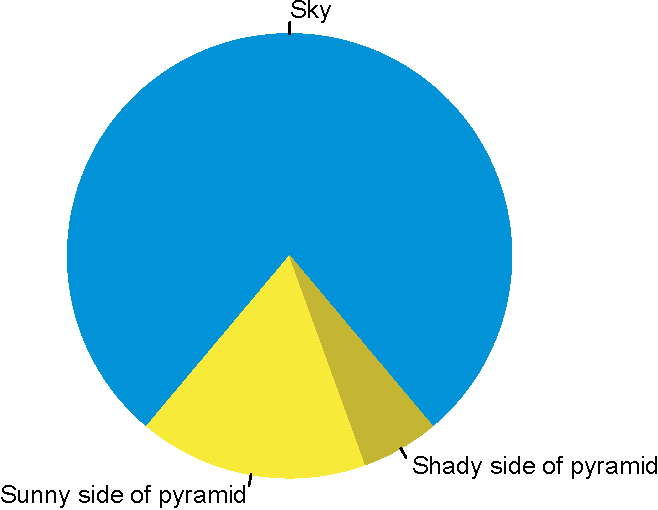
\includegraphics{E_1_files/figure-latex/unnamed-chunk-1-1} \end{center}

\begin{Shaded}
\begin{Highlighting}[]
\FunctionTok{plot}\NormalTok{(cars)}
\FunctionTok{lines}\NormalTok{(}\FunctionTok{lowess}\NormalTok{(cars))}
\end{Highlighting}
\end{Shaded}

\begin{center}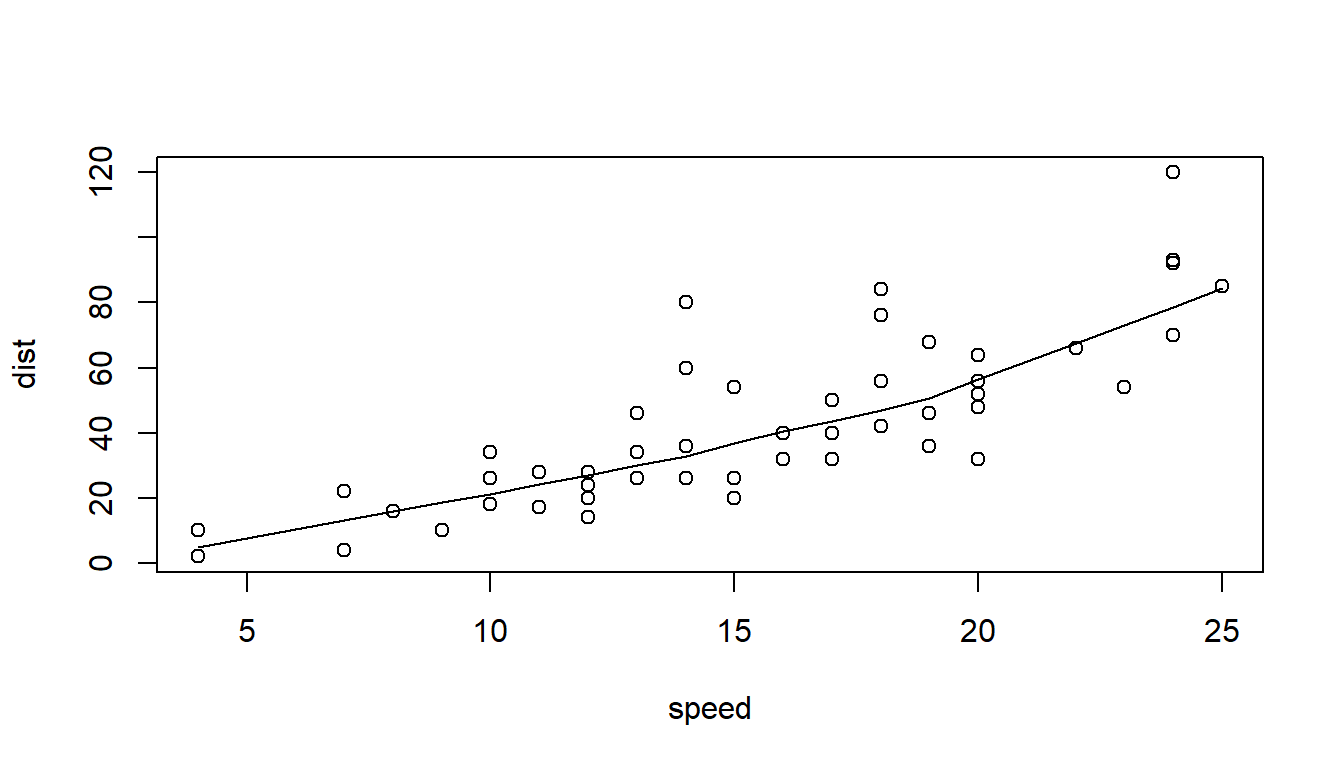
\includegraphics{E_1_files/figure-latex/unnamed-chunk-2-1} \end{center}

\begin{Shaded}
\begin{Highlighting}[]
\FunctionTok{library}\NormalTok{(ggplot2)}
\end{Highlighting}
\end{Shaded}

\begin{verbatim}
## Warning: package 'ggplot2' was built under R version 4.1.3
\end{verbatim}

\begin{Shaded}
\begin{Highlighting}[]
\CommentTok{\# Create data}
\NormalTok{data }\OtherTok{\textless{}{-}} \FunctionTok{data.frame}\NormalTok{(}
  \AttributeTok{name=}\FunctionTok{c}\NormalTok{(}\StringTok{"A"}\NormalTok{,}\StringTok{"B"}\NormalTok{,}\StringTok{"C"}\NormalTok{,}\StringTok{"D"}\NormalTok{,}\StringTok{"E"}\NormalTok{) ,  }
  \AttributeTok{value=}\FunctionTok{c}\NormalTok{(}\DecValTok{3}\NormalTok{,}\DecValTok{12}\NormalTok{,}\DecValTok{5}\NormalTok{,}\DecValTok{18}\NormalTok{,}\DecValTok{45}\NormalTok{)}
\NormalTok{  )}

\CommentTok{\# Barplot}
\FunctionTok{ggplot}\NormalTok{(data, }\FunctionTok{aes}\NormalTok{(}\AttributeTok{x=}\NormalTok{name, }\AttributeTok{y=}\NormalTok{value)) }\SpecialCharTok{+}
  \FunctionTok{geom\_bar}\NormalTok{(}\AttributeTok{stat =} \StringTok{"identity"}\NormalTok{, }\AttributeTok{width=}\FloatTok{0.5}\NormalTok{) }\SpecialCharTok{+}
  \FunctionTok{coord\_flip}\NormalTok{()}
\end{Highlighting}
\end{Shaded}

\begin{center}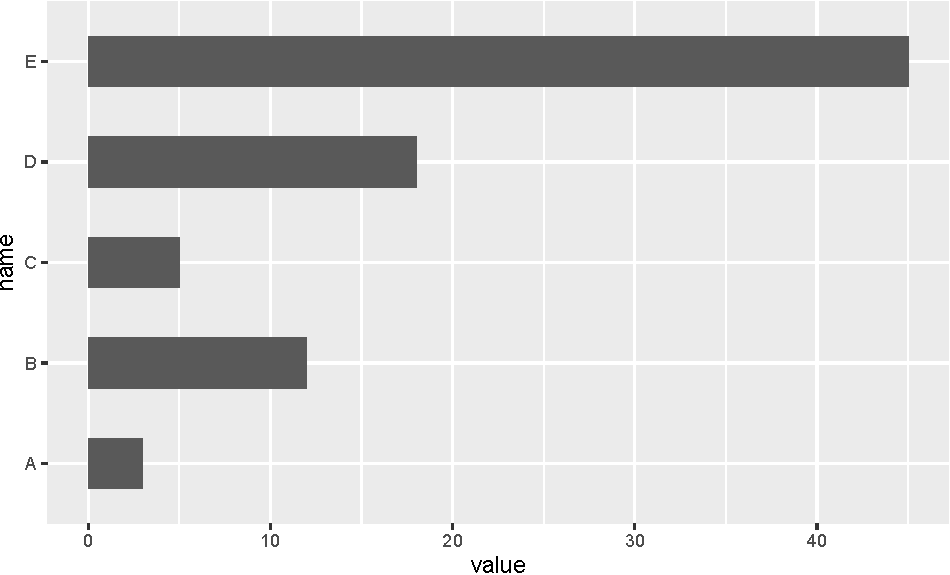
\includegraphics{E_1_files/figure-latex/unnamed-chunk-3-1} \end{center}

\hypertarget{medidas-de-tendencia-central}{%
\chapter{Medidas de tendencia central}\label{medidas-de-tendencia-central}}

Son aquellas medidas que buscan un dato representivo central de un conjunto de datos tales como la media, la moda y la mediana.

\begin{definition}[Datos agrupados y los no agrupados]
\protect\hypertarget{def:tabulacion}{}\label{def:tabulacion}La principal diferencia entre los datos agrupados y los no agrupados es que los agrupados están clasificados según un criterio y los no agrupados se encuentran en el mismo formato que cuando se recopilaron.
\end{definition}

\begin{longtable}[]{@{}cccccc@{}}
\caption{\label{tab:agrupados1} Datos agrupados en intervalos.}\tabularnewline
\toprule
Clase & \(Y_i\) & \(f_i\) & \(F_i\) & \(\ldots\) & \(H_i^*\%\) \\
\midrule
\endfirsthead
\toprule
Clase & \(Y_i\) & \(f_i\) & \(F_i\) & \(\ldots\) & \(H_i^*\%\) \\
\midrule
\endhead
\([y_1,y_2)\) & \(y_1\) & \(f_1\) & \(\ldots\) & \(\ldots\) & \(H_1^*\%\) \\
\([y_2,y_3)\) & \(y_2\) & \(f_2\) & \(\ldots\) & \(\ldots\) & \(H_1^*\%\) \\
\([y_3,y_4)\) & \(y_3\) & \(f_3\) & \(\ldots\) & \(\ldots\) & \(H_1^*\%\) \\
\(\vdots\) & \(\vdots\) & \(\vdots\) & \(\ldots\) & \(\ldots\) & \(\vdots\) \\
\([y_{r-1},y_r]\) & \(y_r\) & \(f_r\) & \(\ldots\) & \(\ldots\) & \(H_1^*\%\) \\
\bottomrule
\end{longtable}

\hypertarget{la-media}{%
\section{La media}\label{la-media}}

A veces llamada \emph{promedio aritmético}, es la medida de tendencia central que pondera los datos.

\hypertarget{media-de-datos-no-agrupados}{%
\subsection{Media de datos no agrupados}\label{media-de-datos-no-agrupados}}

Los datos no están agrupados cuando no están ordenados sobre una tabla de distribución de frecuencias. Sean los \(n\) datos \(x_1, x_2, \ldots, x_n\) entonces la media o promedio aritmético se define como

\[
\overline{x}=\frac{x_1+x_2+\cdots+x_n}{n}=\frac{1}{n}\sum_{i=1}^nx_i
\]

\begin{example}[Media de datos no agrupados]
\protect\hypertarget{exm:media-noagrupados}{}\label{exm:media-noagrupados}wwwwwww
\end{example}

\hypertarget{media-de-datos-agrupados}{%
\subsection{Media de datos agrupados}\label{media-de-datos-agrupados}}

Considérese la siguiente tabla de distribución de frecuencias Tabla \ref{tab:agrupados1} entonces el promedio es \[\overline{x}=\frac{y_1f_1+y_2f_2+\cdots+y_nf_n}{n}=\frac{1}{n}\sum_{i=1}^ny_if_i\]

\begin{example}[Media de datos agrupados]
\protect\hypertarget{exm:media-agrupados}{}\label{exm:media-agrupados}Sean los datos

\begin{longtable}[]{@{}cccc@{}}
\toprule
Clase & \(Y_i\) & \(f_i\) & \(Y_i*f_i\) \\
\midrule
\endhead
\([10,15)\) & 12.5 & 1 & 12.5 \\
\([15,20)\) & 17.5 & 2 & 35 \\
\([20,25)\) & 22.5 & 5 & 112.5 \\
\([25,30)\) & 27.5 & 3 & 82.5 \\
\([30,35]\) & 32.5 & 2 & 65 \\
\(\sum\) & & 13 & 307.5 \\
\bottomrule
\end{longtable}

\[\overline{x}=\frac{12.5+35++112.5+82.5+65}{13}=\frac{307.5}{13}=23.65\]
\end{example}

\begin{exercise}
Si el promedio de \(n\) datos es \(\overline{x}\) entonces el promedio del conjunto inicial más un dato adicional \(x_{n+1}\) es \[\overline{x}'=\frac{n\overline{x}+x_{n+1}}{n+1}\] en general si se adicionan \(r\) datos \(y_1, y_2, \ldots y_r\) entonces el nuevo promedio será \[\overline{x}'=\frac{n\overline{x}+y_{1}+y_2+\ldots+y_r}{n+r}\]
\end{exercise}

\begin{solution}
En efecto sea el promedio
\begin{align*}
\overline{x}'&=\frac{x_1+x_2+\cdots+x_{n+1}}{n+1}\\
&=\frac{n\frac{x_1+x_2+\cdots x_n}{n}+x_{n+1}}{n+1}\\
&=\frac{n\overline{x}+x_{n+1}}{n+1}
\end{align*}
\end{solution}

\hypertarget{la-moda-mo}{%
\section{La moda (Mo)}\label{la-moda-mo}}

\begin{itemize}
\item
  La moda es el valor que tiene mayor frecuencia absoluta.
\item
  Se representa por \(Mo\)
\item
  Si en un grupo hay dos o varias puntuaciones con la misma frecuencia y esa frecuencia es la máxima, entonces la distribución es bimodal es decir, tiene varias modas.
\item
  Cuando todas las puntuaciones de un grupo tienen la misma frecuencia, no hay moda.
\item
  Se puede hallar la moda para variables cualitativas y cuantitativas.
\item
  Cuando todas las puntuaciones de un grupo tienen la misma frecuencia, no hay moda.
\item
  Si dos puntuaciones adyacentes tienen la frecuencia máxima, la moda es el promedio de las dos puntuaciones adyacentes.
\item
  Si dos puntuaciones adyacentes tienen la frecuencia máxima, la moda es el promedio de las dos puntuaciones adyacentes.Ejemplos de ejercicios de moda
\end{itemize}

\hypertarget{moda-de-datos-no-tabulados}{%
\subsection{Moda de datos no tabulados}\label{moda-de-datos-no-tabulados}}

En este caso es dato que más repite en un conjunto de datos dados.

La moda es el dato que más se repite por ejemplo sea el conjunto de datos \(x_1\), \(x_2\), \(x_2\), \(x_2\), \(x_3\) entonces la moda es \(\text{Mo}=x_2\)

Halle la moda de los siguinetes datos 3, 5,3,6,7,3,4,5,5 ya que hay hay precencia de dotas que se repiten dos veces en tonces este conjunto de datos recibe el nombre de datos bimodal Mo=3 y Mo=5

\hypertarget{moda-de-datos-tabulados}{%
\subsection{Moda de datos tabulados}\label{moda-de-datos-tabulados}}

La moda es el dato que más se repite por ejemplo sea el conjunto de datos tabulados de la Tabla \ref{tab:agrupados1} entonces la moda es \[ M_o=L_i+\frac{f_i-f_{i-1}}{(f_i-f_{i-1})+(f_i-f_{i+1})}\cdot a_i\]

\begin{itemize}
\item
  \(L_i\) es el límite inferior de la clase modal
\item
  \(f_i\) es la frecuencia absoluta de la clase modal
\item
  \(f_{i-1}\) es la frecuencia absoluta inmediatamente inferior a la clase modal
\item
  \(f_{i+1}\) es la frecuencia absoluta inmediatamente posterior a la clase modal
\item
  \(a_i\) es la amplitud de la clase
\end{itemize}

\begin{example}
Sea la tabla

\begin{longtable}[]{@{}cc@{}}
\toprule
Clase & \(f_i\) \\
\midrule
\endhead
\([10,15)\) & 2 \\
\([15,20)\) & 5 \\
\([20,25)\) & 10 \\
\([25,30)\) & 3 \\
\([30,35]\) & 1 \\
\bottomrule
\end{longtable}

Primeramente la mayor frecuencia absoluta es 10 y corresponde \(f_3=10\) por tanto \(i=3\). \(L_i=20\)

\[ M_o=L_i+\frac{f_i-f_{i-1}}{(f_i-f_{i-1})+(f_i-f_{i+1})}\cdot a_i=\] \[ =20+\frac{10-5}{(10-5)+(10-3)}\cdot 5=20+\frac{5}{12}*5=22.08\]

\href{https://www.superprof.es/apuntes/escolar/matematicas/estadistica/descriptiva/moda-estadistica.html}{Más información}
\end{example}

\hypertarget{la-mediana-me}{%
\section{La mediana (Me)}\label{la-mediana-me}}

\hypertarget{mediana-de-datos-no-tabulados}{%
\subsection{Mediana de datos no tabulados}\label{mediana-de-datos-no-tabulados}}

Obtener la mediana consiste en ordenar los datos de menor a mayor y considerar dos casos: El primero si el número de datos es impar entonces el dato \(x_{\frac{n+1}{2}}\) del conjunto ordenado será la mediana es decir \[\text{Me}=x_{\frac{n+1}{2}}\] de otro lado si el número de datos es par entonces la mediana es la semisuma de los dos datos intermedios es decir \[\text{Me}=\frac{x_{\frac{n}{2}}+x_{\frac{n}{2}+1}}{2}\]

\begin{example}
Sean los conjuntos de datos 5, 6, 8, 2, 1, 5, 6, 7, 10, 0, 14 y 20, 25, 6, 5, 19, 5 obtener la mediana de estos conjuntos de datos.

Al ordenarlos se obtiene el siguiente arreglo 0, 1, 2, 5, 5, 6, 6, 7, 8, 10, 14 y considerando que \(x_1=0\), \(x_2=1\), \(\ldots\), \(x_{11}=14\) en este caso el número de datos es impar entonces el dato \(x_{\frac{11+1}{2}}=x_{6}=6\) el la mediana. De otro lado el segundo conjunto de datos al ser ordenados 5, 5, 6, 19, 20, 25 ademas considerando que \(x_1=5\), \(x_2=5\), \(\ldots\), \(x_6=25\) conducen a obtener la mediana \(\text{Me}=\frac{x_{\frac{6}{2}}+x_{\frac{6}{2}+1}}{2}=\frac{6+19}{2}=12.5\).
\end{example}

\hypertarget{mediana-de-datos-tabulados}{%
\subsection{Mediana de datos tabulados}\label{mediana-de-datos-tabulados}}

La mediana se encuentra en el intervalo donde la frecuencia acumulada llega hasta la mitad de la suma de las frecuencias absolutas. Sea la Tabla \ref{tab:agrupados1}.

Es decir tenemos que buscar el intervalo en el que se encuentre.

\[  M_e=L_{i}+\frac{\frac{N}{2}-F_{i-1}}{f_{i}}\cdot a_{i}\]

\(L_{i}\) es el límite inferior de la clase donde se encuentra la mediana

\(\frac{N}{2}\) es la semisuma de las frecuencias absolutas

\(f_{i}\) es la frecuencia absoluta de la clase mediana

\(F_{i-1}\) es la frecuencia acumulada anterior a la clase mediana

\(a_{i}\) es la amplitud de la clase

La mediana es independiente de las amplitudes de los intervalos

\href{https://www.superprof.es/apuntes/escolar/matematicas/estadistica/descriptiva/mediana.html}{Más información}

\begin{example}
Sea la tabla

\begin{longtable}[]{@{}ccc@{}}
\toprule
Clase & \(f_i\) & \(F_i\) \\
\midrule
\endhead
\([10,15)\) & 1 & 1 \\
\([15,20)\) & 2 & 3 \\
\([20,25)\) & 5 & 8 \\
\([25,30)\) & 3 & 11 \\
\([30,35]\) & 1 & 12 \\
\(\sum\) & 12 & \\
\bottomrule
\end{longtable}

\[\frac{N}{2}=12/2=6\] ubicando en las frecuencias absolutas acumuladas que corresponde al intervalo \([20,25)\)

\[  M_e=L_{i}+\frac{\frac{N}{2}-F_{i-1}}{f_{i}}\cdot a_{i}\] \[  =20+\frac{\frac{12}{2}-3}{5}\cdot 5=23\] por lo tanto la mediana de este conjunto de datos tabulados (agrupados) es \(Me=23\)
\end{example}

\hypertarget{asignaciuxf3n}{%
\section{Asignación}\label{asignaciuxf3n}}

Halle le media, la moda y la mediana de los siguientes datos tabulados

\begin{longtable}[]{@{}cccc@{}}
\toprule
Clase & \(Y_i\) & \(f_i\) & \(F_i\) \\
\midrule
\endhead
\([100,150)\) & & 1 & 1 \\
\([150,200)\) & & 2 & 3 \\
\([200,250)\) & & 5 & \\
\([250,300)\) & & 7 & \\
\([300,350]\) & & 10 & \\
\([350,400]\) & & 6 & \\
\([400,450]\) & & 5 & \\
\([450,500]\) & & 2 & \\
\([500,550]\) & & 1 & \\
\bottomrule
\end{longtable}

\[\overline{x}=\frac{y_1f_1+y_2f_2+\cdots+y_nf_n}{n}=\frac{1}{n}\sum_{i=1}^ny_if_i\]

\[ M_o=L_i+\frac{f_i-f_{i-1}}{(f_i-f_{i-1})+(f_i-f_{i+1})}\cdot a_i\]

\[  M_e=L_{i}+\frac{\frac{N}{2}-F_{i-1}}{f_{i}}\cdot a_{i}\]

\hypertarget{medidas-de-dispersiuxf3n}{%
\chapter{Medidas de dispersión}\label{medidas-de-dispersiuxf3n}}

Son medidas o parametros que miden la dispersion de los datos, entre ellos tenmos

\hypertarget{rango}{%
\section{Rango}\label{rango}}

Es la longitud de un conjunto de datos, es decir la diferencia
\[R=x_{max}-x_{min}\]

Por ejemplo sean los datos 2, 5, 6, 1, 7, 5, 8, 6
tiene el dato máximo \(x_{max}=8\) y el dato mínimo \(x_{min}=1\). Por lo tanto \(R=x_{max}-x_{min}=8-1=7.\)

\hypertarget{varianza}{%
\section{Varianza}\label{varianza}}

Mide la dispersión de los datso con respecto a la media

\hypertarget{datos-no-tabulados}{%
\subsection{Datos no tabulados}\label{datos-no-tabulados}}

Se usa la siguiente fórmula
\[s^2=\frac{\sum\left(x_i-\overline{x}\right )^2}{n-1}\]

Ejemplo. Sean los datos 2, 5, 6, 1, 7, 5, 8, 6

\[\overline{x}=40/8=5\]

\[
\begin{aligned}
s^2&=\frac{\sum\left(x_i-\overline{x}\right )^2}{n-1}\\
&=\frac{\left(x_1-\overline{x}\right )^2+\left(x_2-\overline{x}\right )^2+\left(x_3-\overline{x}\right )^2+\left(x_4-\overline{x}\right )^2+\left(x_5-\overline{x}\right )^2+\left(x_6-\overline{x}\right )^2+\left(x_7-\overline{x}\right )^2+\left(x_8-\overline{x}\right )^2}{8-1}\\
&=\frac{\left(2-5\right )^2+\left(5-5\right )^2+\left(6-5\right )^2+\left(1-5\right )^2+\left(7-5\right )^2+\left(5-5\right )^2+\left(8-5\right )^2+\left(6-5\right )^2}{8-1}\\
&=\frac{9+0+1+16+4+0+9+1}{7}\\
&=\frac{40}{7}=5.71
\end{aligned}
\]

\hypertarget{datos-tabulados}{%
\subsection{Datos tabulados}\label{datos-tabulados}}

Sea la Tabla \ref{tab:agrupados1}. Entonces la formula que resuelve la varianza es
\[s^2=\frac{\sum f_i\left(Y_i-\overline{x}\right )^2}{n-1}\]

\(\overline{x}=\frac{\sum Y_i*f_i}{n}=747.5/31=24.11\)

\begin{longtable}[]{@{}cccc@{}}
\toprule
Clase & \(Y_i\) & \(f_i\) & \(Y_i*f_i\) \\
\midrule
\endhead
\([5,10)\) & 7.5 & 1 & 7.5 \\
\([10,15)\) & 12.5 & 2 & 25 \\
\([15,20)\) & 17.5 & 5 & 87.5 \\
\([20,25)\) & 22.5 & 7 & 157.5 \\
\([25,30]\) & 27.5 & 10 & 275 \\
\([30,35]\) & 32.5 & 6 & 195 \\
\(\sum\) & & 31 & \\
\bottomrule
\end{longtable}

Por lo tanto la varianza para datos agrupados es

\[
\begin{aligned}
s^2&=\frac{\sum f_i\left(Y_i-\overline{x}\right )^2}{n-1}\\
&=\frac{f_1\left(Y_1-\overline{x}\right )^2+f_2\left(Y_2-\overline{x}\right )^2+f_3\left(Y_3-\overline{x}\right )^2+f_4\left(Y_4-\overline{x}\right )^2+f_5\left(Y_5-\overline{x}\right )^2+f_6\left(Y_6-\overline{x}\right )^2}{31-1}\\
&=\frac{1\left(7.5-24.11\right )^2+2\left(12.5-24.11\right )^2+5\left(17.5-24.11\right )^2+7\left(22.5-24.11\right )^2+10\left(27.5-24.11\right )^2+6\left(32.5-24.11\right )^2}{31-1}
\\
&=\frac{1*275.89+2*134.79+5*43.69+7*2.59+10*11.49+6*7.39}{31-1}
\\
&=\frac{275.89+269.58+218.45+18.13+114.9+44.34}{30}\\
&=\frac{941.29}{30}=31.38
\end{aligned}
\]

Por lo tanto \[s^2=  31.38\]

\hypertarget{desviaciuxf3n-tuxedpica}{%
\section{Desviación típica}\label{desviaciuxf3n-tuxedpica}}

\[s=\sqrt{s^2}\]

La desviacion típica o estandar del siguiente conjunto de datos tabulados

\begin{longtable}[]{@{}cccc@{}}
\toprule
Clase & \(Y_i\) & \(f_i\) & \(Y_i*f_i\) \\
\midrule
\endhead
\([5,10)\) & 7.5 & 1 & 7.5 \\
\([10,15)\) & 12.5 & 2 & 25 \\
\([15,20)\) & 17.5 & 5 & 87.5 \\
\([20,25)\) & 22.5 & 7 & 157.5 \\
\([25,30]\) & 27.5 & 10 & 275 \\
\([30,35]\) & 32.5 & 6 & 195 \\
\(\sum\) & & 31 & \\
\bottomrule
\end{longtable}

es \[s=\sqrt{s^2}=\sqrt{31.38}=5.60\]

\hypertarget{desviaciuxf3n-media-absoluta}{%
\section{Desviación media absoluta}\label{desviaciuxf3n-media-absoluta}}

\hypertarget{datos-no-tabulados-1}{%
\subsection{Datos no tabulados}\label{datos-no-tabulados-1}}

\[DM=\frac{1}{n}\sum \left\vert x_i-\overline{x}\right\vert\]

Sean los datos 2, 5, 6, 1, 7, 5, 8, 6

\[\overline{x}=40/8=5\]

Entonces

\[
\begin{aligned}
DM&=\frac{\sum\left\vert x_i-\overline{x}\right \vert}{n}\\
&=... Resolver
\end{aligned}
\]

\hypertarget{datos-tabulados-1}{%
\subsection{Datos tabulados}\label{datos-tabulados-1}}

\[DM=\frac{1}{n}\sum f_i \left \vert Y_i-\overline{x}\right\vert\]

\(y_i\) marca de clase o punto medio de la clase \(i\)

\(\overline{x}=\frac{\sum Y_i*f_i}{n}=747.5/31=24.11\)

\begin{longtable}[]{@{}cccc@{}}
\toprule
Clase & \(Y_i\) & \(f_i\) & \(Y_i*f_i\) \\
\midrule
\endhead
\([5,10)\) & 7.5 & 1 & 7.5 \\
\([10,15)\) & 12.5 & 2 & 25 \\
\([15,20)\) & 17.5 & 5 & 87.5 \\
\([20,25)\) & 22.5 & 7 & 157.5 \\
\([25,30]\) & 27.5 & 10 & 275 \\
\([30,35]\) & 32.5 & 6 & 195 \\
\(\sum\) & & 31 & \\
\bottomrule
\end{longtable}

Por lo tanto la desviación media absoluta es

\[
\begin{aligned}
DM&=\frac{\sum f_i\left \vert Y_i-\overline{x}\right \vert}{n}\\
&=\frac{f_1\left\vert Y_1-\overline{x}\right \vert +f_2\left\vert Y_2-\overline{x}\right \vert +f_3\left\vert Y_3-\overline{x}\right \vert +f_4\left\vert Y_4-\overline{x}\right \vert +f_5\left\vert Y_5-\overline{x}\right \vert +f_6\left\vert Y_6-\overline{x}\right \vert }{31}\\
&=\frac{1\left\vert 7.5-24.11\right \vert +2\left\vert 12.5-24.11\right \vert +5\left\vert 17.5-24.11\right \vert +7\left\vert 22.5-24.11\right \vert +10\left\vert 27.5-24.11\right \vert +6\left\vert 32.5-24.11\right \vert }{31}\\
&=\frac{1*16.61 +2*11.61 +5*6.61 +7*1.61 +10*3.39 +6*8.39 }{31}\\
\\
&=\frac{277.33}{31}=8.94\\
\end{aligned}
\]

por lo tanto \[DM=8.94\]

\hypertarget{desviaciuxf3n-mediana-absoluta}{%
\section{Desviación mediana absoluta}\label{desviaciuxf3n-mediana-absoluta}}

\hypertarget{datos-no-tabulados-2}{%
\subsection{Datos no tabulados}\label{datos-no-tabulados-2}}

\[DMe=\frac{1}{n}\sum \left\vert Y_i-Me\right\vert\]

Sean los datos 2, 5, 6, 1, 7, 5, 8, 6 (Ejercicio)

\hypertarget{datos-tabulados-2}{%
\subsection{Datos tabulados}\label{datos-tabulados-2}}

\[DMe=\frac{1}{n}\sum f_i \left \vert Y_i-Me\right\vert\]

\(Me=?\) (Ejercicio)

\begin{longtable}[]{@{}cccc@{}}
\toprule
Clase & \(Y_i\) & \(f_i\) & \(Y_i*f_i\) \\
\midrule
\endhead
\([5,10)\) & 7.5 & 2 & 7.5 \\
\([10,15)\) & 12.5 & 3 & 25 \\
\([15,20)\) & & 4 & 87.5 \\
\([20,25)\) & 22.5 & 7 & 157.5 \\
\([25,30]\) & 27.5 & 10 & 275 \\
\([30,35]\) & & 8 & 195 \\
\(\sum\) & & & \\
\bottomrule
\end{longtable}

Por lo tanto la desviacion de la mediana absoluta es

(Ejercicio)

\[
\begin{aligned}
s^2&=\frac{\sum f_i\left \vert Y_i-Me\right \vert}{n}\\
&=\frac{f_1\left(Y_1-Me\right )^2+f_2\left(Y_2-Me\right )^2+f_3\left(Y_3-Me\right )^2+f_4\left(Y_4-Me\right )^2+f_5\left(Y_5-Me\right )^2+f_6\left(Y_6-Me\right )^2}{31}\\
&=complete
\end{aligned}
\]

\hypertarget{coeficiente-de-variacion}{%
\section{Coeficiente de variacion}\label{coeficiente-de-variacion}}

\[Cv=\frac{s}{\overline{x}}\cdot 100\] Si \(Cv>25\%\) se dice que los datos estan muy dispersos Si \(Cv<25\%\) se dice que los datos estan muy juntos

Para el conjunto de datos

\begin{longtable}[]{@{}cccc@{}}
\toprule
Clase & \(Y_i\) & \(f_i\) & \(Y_i*f_i\) \\
\midrule
\endhead
\([5,10)\) & 7.5 & 1 & 7.5 \\
\([10,15)\) & 12.5 & 2 & 25 \\
\([15,20)\) & 17.5 & 5 & 87.5 \\
\([20,25)\) & 22.5 & 7 & 157.5 \\
\([25,30]\) & 27.5 & 10 & 275 \\
\([30,35]\) & 32.5 & 6 & 195 \\
\(\sum\) & & 31 & \\
\bottomrule
\end{longtable}

\[Cv=\frac{5.60}{24.11}\cdot 100=0.23\cdot 100=23\%\]

\hypertarget{asignaciuxf3n-1}{%
\section{Asignación}\label{asignaciuxf3n-1}}

Halle el rango, la varianza, la desviación típica, desviación media, desviación mediana absoluta y el coeficiente de variación. Grafique el hstograma y ubique estos estadigrafos

\begin{longtable}[]{@{}cccc@{}}
\toprule
Clase & \(Y_i\) & \(f_i\) & \(F_i\) \\
\midrule
\endhead
\([50,100)\) & & 8 & 1 \\
\([100,150)\) & & 20 & 3 \\
\([150,200)\) & & 50 & \\
\([200,250)\) & & 70 & \\
\([250,300]\) & & 100 & \\
\([300,350]\) & & 60 & \\
\(\sum\) & & 20 & \\
\bottomrule
\end{longtable}

\hypertarget{medidas-de-posicion-cuantiles}{%
\chapter{Medidas de posicion (cuantiles)}\label{medidas-de-posicion-cuantiles}}

\begin{itemize}
\tightlist
\item
  Los deciles, que dividen a la distribución en diez partes;
\item
  Los percentiles, que dividen a la distribución en cien partes.
\end{itemize}

\hypertarget{cuartiles}{%
\section{Cuartiles}\label{cuartiles}}

Los cuartiles, que dividen a la distribución en cuatro partes (corresponden a los cuantiles 0,25; 0,50 y 0,75); \(Q_1, Q_2, Q_3\)

\hypertarget{datos-no-agrupados}{%
\subsection{Datos no agrupados}\label{datos-no-agrupados}}

Sean los datos 1, 2, 5, 1 ,5, 6, 7, 8, 9, 3, 4, 5, 2, 6, 2, 5, 6, 7 Ordenar de menor a mayor (creciente)

Si \[Q_k=\frac{k(n+1)}{4}\] es entero entonces el cuartil es el dato de la posicion \(Q_k=x_\frac{k(n+1)}{4}\) en caso contrario se interpola los datos extremos donde se encuentra el valor \(Q_k\)

\begin{itemize}
\tightlist
\item
  Ejemplo 1, 2, 5, 1 ,5, 6, 7, 8, 9, 3, 4, 5, 2, 6, 2, 5, 6, 7 ordenados de menor a mayor 1, 1, 2, 2, 2, 3, 4, 5, 5, 5, 5, 6, 6, 6, 7, 7, 8, 9
\end{itemize}

\(Q_1=\frac{1(18+1)}{4}=4.75\) interpolando \(Q_1=2+(2-2)\cdot 0.75=2\)

\(Q_2=\frac{2(18+1)}{4}=9.5\) interpolando \(Q_2=5+(5-5)\cdot 0.5=5\)

\(Q_3=\frac{3(18+1)}{4}=14.25\) interpolando \(Q_3=6+(7-6)\cdot 0.25=6.25\)

\hypertarget{datos-agrupados}{%
\subsection{Datos agrupados}\label{datos-agrupados}}

\[Q_k=L_i+ A\left(\frac{\frac{kn}{4}-F_{i-1}}{F_i-F_{i-1}}\right);k=1,2,3\]

\begin{itemize}
\tightlist
\item
  \(L_i\) limite inferior del intervalo que contiene al decil
\item
  \(F_{i-1}\) frecuencia acumulada en la clase anterior al decil
\item
  \(F_i\) frecuencia acumulada en la clase al decil
\item
  \(A\) amplitud intervalica
\item
  \(n\) numero de datos
\item
  \(k\) indice del cuartil correspondiente
\end{itemize}

\[
\begin{aligned}
Q_1&=L_i+ A\left(\frac{\frac{1n}{4}-F_{i-1}}{F_i-F_{i-1}}\right)\\
&=L_i+ A\left(\frac{\frac{1*39}{4}-F_{i-1}}{F_i-F_{i-1}}\right)\\
&=20+ 5\cdot\left(\frac{9.75 -8}{15-8}\right)\\
&=21.5
\end{aligned}
\]

\[
\begin{aligned}
Q_2&=L_i+ A\left(\frac{\frac{2n}{4}-F_{i-1}}{F_i-F_{i-1}}\right)\\
&=L_i+ A\left(\frac{\frac{2*39}{4}-F_{i-1}}{F_i-F_{i-1}}\right)\\
&=25+ 5\cdot\left(\frac{19.5 -15}{25-15}\right)\\
&= 27.5
\end{aligned}
\]

\[
\begin{aligned}
Q_3&=L_i+ A\left(\frac{\frac{3n}{4}-F_{i-1}}{F_i-F_{i-1}}\right)\\
&=L_i+ A\left(\frac{\frac{2*39}{4}-F_{i-1}}{F_i-F_{i-1}}\right)\\
&=30+ 5\cdot\left(\frac{29.25 -25}{31-25}\right)\\
&= 33.542
\end{aligned}
\]

\begin{longtable}[]{@{}cccc@{}}
\toprule
Clase & \(Y_i\) & \(f_i\) & \(F_i\) \\
\midrule
\endhead
\([5,10)\) & 7.5 & 1 & 1 \\
\([10,15)\) & 12.5 & 2 & 3 \\
\([15,20)\) & 17.5 & 5 & 8 \\
\([20,25)\) & 22.5 & 7 & 15 \\
\([25,30]\) & 27.5 & 10 & 25 \\
\([30,35]\) & 32.5 & 6 & 31 \\
\([35,40]\) & 37.5 & 5 & 36 \\
\([40,45]\) & 42.5 & 3 & 39 \\
\(\sum\) & & 39 & \\
\bottomrule
\end{longtable}

\hypertarget{quintiles}{%
\section{Quintiles}\label{quintiles}}

wwwwwwwww

\hypertarget{deciles}{%
\section{Deciles}\label{deciles}}

Los deciles, que dividen a la distribución en diez partes es decir \(D_1, D_2,\ldots, D_9\)

\hypertarget{datos-no-agrupados-1}{%
\subsection{Datos no agrupados}\label{datos-no-agrupados-1}}

Sean los datos 1, 2, 5, 1 ,5, 6, 7, 8, 9, 3, 4, 5, 2, 6, 2, 5, 6, 7 Ordenar de menor a mayor (creciente)

Si \[D_k=\frac{k(n+1)}{10}\] es entero entonces el decil es el dato de la posicion \(D_k=x_\frac{k(n+1)}{10}; k=1, 2, 3, \ldots, 9\) Si \[D_k=\frac{k(n+1)}{10}\] no es entero entonces el decil es la interpolacion lineal de de los dos valores entre las cuales se encuentra \(D_k=\frac{k(n+1)}{10}\)

\begin{itemize}
\tightlist
\item
  Ejemplo 1, 2, 5, 1 ,5, 6, 7, 8, 9, 3, 4, 5, 2, 6, 2, 5, 6, 7 ordenados de menor a mayor 1, 1, 2, 2, 2, 3, 4, 5, 5, 5, 5, 6, 6, 6, 7, 7, 8, 9 entonces
\end{itemize}

\[D_9=\frac{9(18+1)}{10}=17.1\] interpolando el decil 9 es \(D_9=8+(9-8)\cdot 0.1=8.1\)

\hypertarget{datos-agrupados-1}{%
\subsection{Datos agrupados}\label{datos-agrupados-1}}

\[D_k=L_i+ A\left(\frac{\frac{kn}{10}-F_{i-1}}{F_i-F_{i-1}}\right)\]

\begin{longtable}[]{@{}cccc@{}}
\toprule
Clase & \(Y_i\) & \(f_i\) & \(F_i\) \\
\midrule
\endhead
\([5,10)\) & 7.5 & 1 & 1 \\
\([10,15)\) & 12.5 & 2 & 3 \\
\([15,20)\) & 17.5 & 5 & 8 \\
\([20,25)\) & 22.5 & 7 & 15 \\
\([25,30]\) & 27.5 & 10 & 25 \\
\([30,35]\) & 32.5 & 6 & 31 \\
\([35,40]\) & 37.5 & 5 & 36 \\
\([40,45]\) & 42.5 & 3 & 39 \\
\(\sum\) & & 39 & \\
\bottomrule
\end{longtable}

\[D_9=L_i+ A\left(\frac{\frac{9\cdot 39}{10}-F_{i-1}}{F_i-F_{i-1}}\right)\]

Entonces \(\frac{9\cdot 39}{10}=35.1\)

\[D_9=35+ 5\left(\frac{35.1-31}{36-31}\right)=39.1\]

\hypertarget{percentiles}{%
\section{Percentiles}\label{percentiles}}

Los percentiles, que dividen a la distribución en diez partes es decir \(P_1, P_2,\ldots, P_{99}\)

\hypertarget{datos-no-agrupados-2}{%
\subsection{Datos no agrupados}\label{datos-no-agrupados-2}}

Si \[P_k=\frac{k(n+1)}{100}; k=1, 2,  \ldots, 99\] es entero entonces el cuartil es el dato de la posicion \(P_k=x_\frac{k(n+1)}{100}\) Si \[P_k=\frac{k(n+1)}{100}\] no es entero entonces el cuartil es la interpolacion lineal de de los dos valores entre las cuales se encuentra \(Q_k=\frac{k(n+1)}{100}\)

\begin{itemize}
\tightlist
\item
  Ejemplo 1, 2, 5, 1 ,5, 6, 7, 8, 9, 3, 4, 5, 2, 6, 2, 5, 6, 7 Al ordenar de manera creciente 1, 2, 5, 1 ,5, 6, 7, 8, 9, 3, 4, 5, 2, 6, 2, 5, 6, 7 y \[P_k=\frac{k(18+1)}{100}\]
\end{itemize}

\hypertarget{datos-agrupados-2}{%
\subsection{Datos agrupados}\label{datos-agrupados-2}}

\[P_k=L_i+ A\left(\frac{\frac{kn}{100}-F_{i-1}}{F_i-F_{i-1}}\right)=\int_1^3f(x)\]

\begin{longtable}[]{@{}cccc@{}}
\toprule
Clase & \(Y_i\) & \(f_i\) & \(F_i\) \\
\midrule
\endhead
\([5,10)\) & 7.5 & 1 & 1 \\
\([10,15)\) & 12.5 & 2 & 3 \\
\([15,20)\) & 17.5 & 5 & \\
\([20,25)\) & 22.5 & 7 & \\
\([25,30]\) & & 10 & \\
\([30,35]\) & & 6 & \\
\([35,40]\) & & 5 & \\
\([40,45]\) & & 3 & \\
\(\sum\) & & 2 & \\
\bottomrule
\end{longtable}

\hypertarget{medidas-de-asimetruxeda}{%
\chapter{Medidas de asimetría}\label{medidas-de-asimetruxeda}}

Podemos decir que la asimetría indica cuánto se desvía nuestra distribución subyacente de la \textbf{distribución normal}, ya que la distribución normal tiene \textbf{asimetría 0}. Generalmente, tenemos \textbf{tres tipos de asimetría}.

\begin{enumerate}
\def\labelenumi{\arabic{enumi}.}
\item
  \textbf{Desviación simétrica}: cuando la asimetría es cercana a 0 y la media es casi la misma que la mediana
\item
  \textbf{Desviación negativa}: cuando la cola izquierda del histograma de la distribución es más larga y la mayoría de las observaciones se concentran en la cola derecha. En este caso, también podemos utilizar el término ``sesgado a la izquierda'' o ``cola izquierda''. y la \textbf{mediana es mayor que la media}.
\item
  \textbf{Desviación positiva}: cuando la cola derecha del histograma de la distribución es más larga y la mayoría de las observaciones se concentran en la cola izquierda. En este caso, también podemos usar el término ``sesgado a la derecha'' o ``cola derecha''. y la \textbf{mediana es menor que la media}.

  \begin{figure}
  \centering
  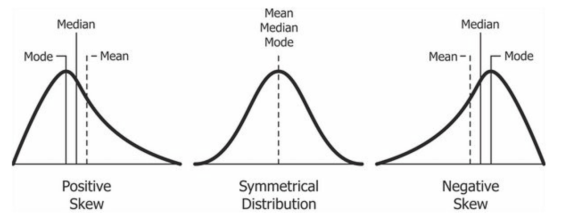
\includegraphics{simetria.png}
  \caption{Medidas de asimetría}
  \end{figure}
\end{enumerate}

\begin{itemize}
\tightlist
\item
  Índice de simetría de \textbf{Pearson}:
\end{itemize}

\[
 f_1=\frac{\overline{x}-Mo}{\sigma}
 \]

\begin{itemize}
\tightlist
\item
  Índice de simetría de \textbf{Fisher}:
\end{itemize}

\[
f_2=\frac{\sum_{i=1}^{n}\left( x_i-\overline{x}\right)^3}{n\sigma^3}
\]

\begin{verbatim}
* Simétrico : valores entre -0,5 y 0,5
* Datos asimétricos moderados : valores entre -1 y -0,5 o entre 0,5 y 1
* Datos muy sesgados : valores menores que -1 o mayores que 1
\end{verbatim}

Si la distribución es simétrica, ambos índices son iguales a 0; si es asimétrica a la derecha, ambos son positivos; y si es asimétrica a la izquierda, ambos índices son negativos.

\hypertarget{normal-simuxe9trica}{%
\section{Normal: Simétrica}\label{normal-simuxe9trica}}

wwwwwwwwwwwwwwwwwwwwwwww

\begin{verbatim}
## [1] 0.5059805
\end{verbatim}

\begin{verbatim}
## [1] 78.53333
\end{verbatim}

\begin{center}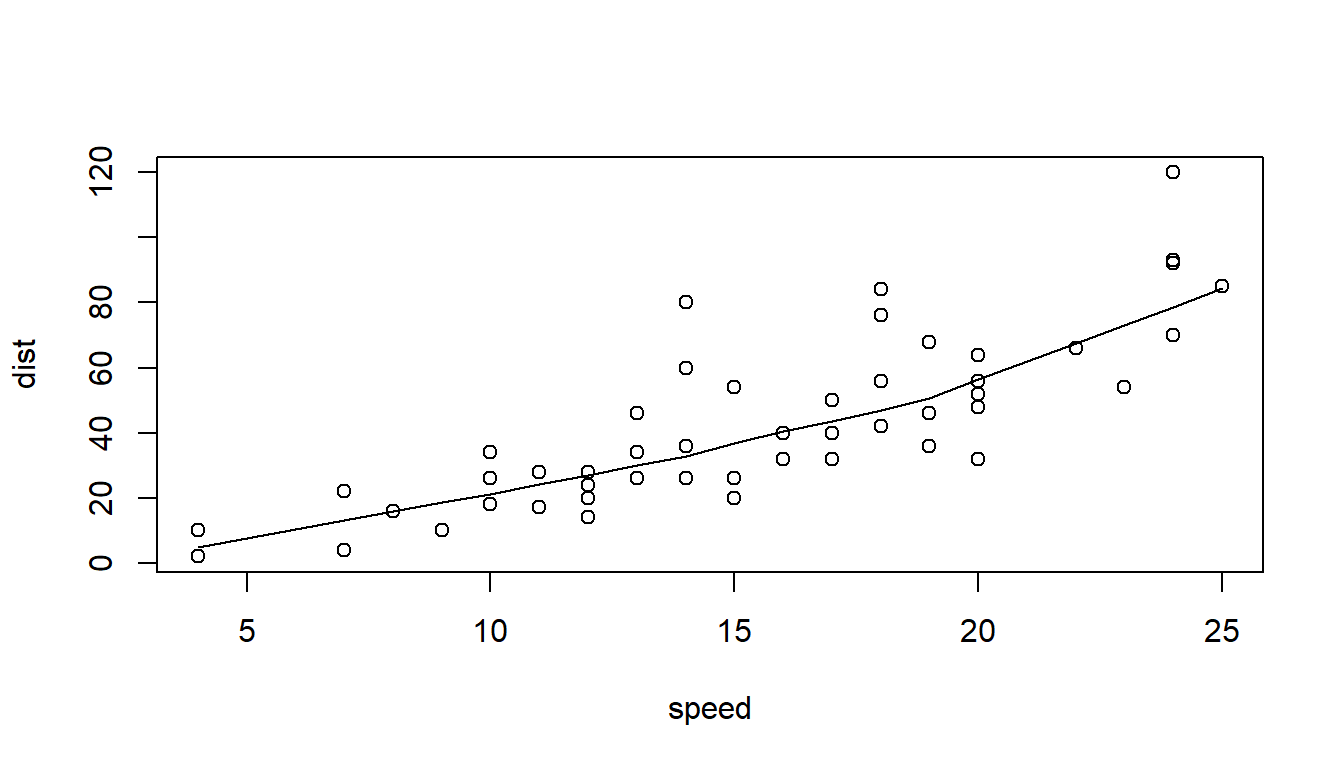
\includegraphics{E_1_files/figure-latex/unnamed-chunk-4-1} \end{center}

\hypertarget{normal-simetruxeda-positiva}{%
\section{Normal: Simetría positiva}\label{normal-simetruxeda-positiva}}

wwwwwwwwwwwwwwwww

\begin{center}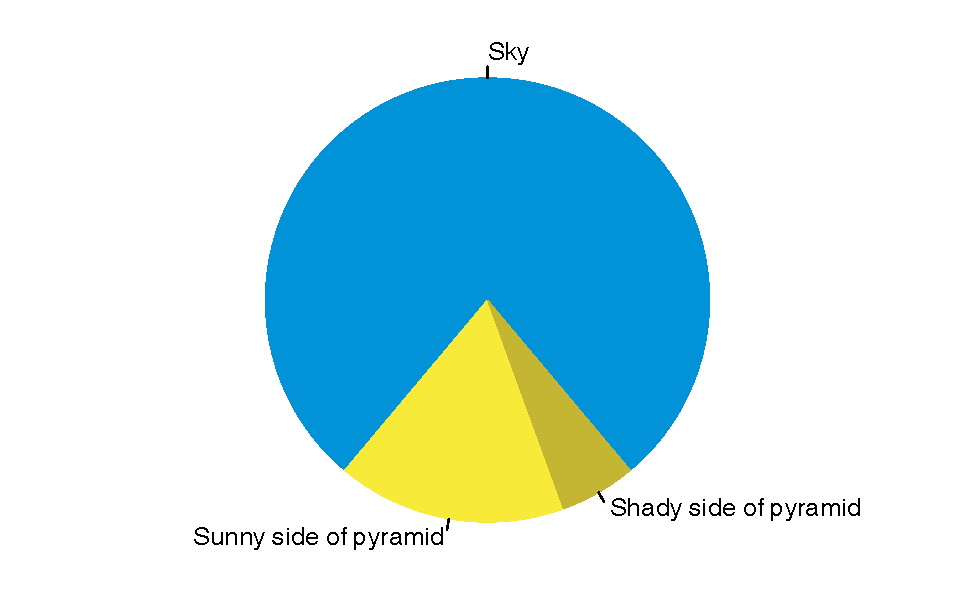
\includegraphics{E_1_files/figure-latex/unnamed-chunk-5-1} \end{center}

\begin{verbatim}
## [1] 1.216579
\end{verbatim}

\hypertarget{normal-simetruxeda-negativa}{%
\section{Normal: Simetría negativa}\label{normal-simetruxeda-negativa}}

wwwwwwwwwwwwwwwww

\begin{center}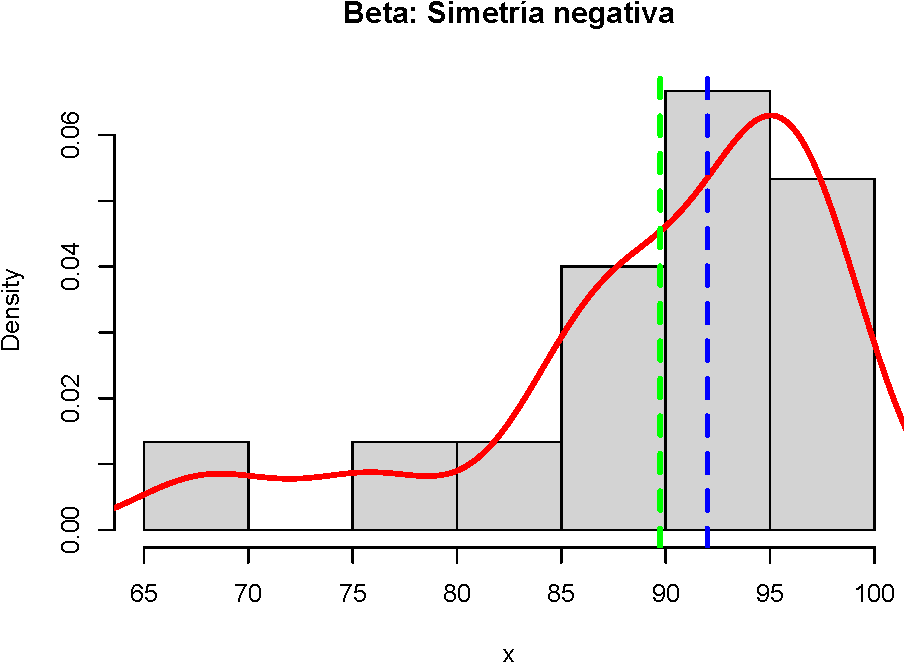
\includegraphics{E_1_files/figure-latex/unnamed-chunk-6-1} \end{center}

\begin{verbatim}
## [1] -1.340429
\end{verbatim}

\begin{longtable}[]{@{}cccc@{}}
\toprule
Clase & \(Y_i\) & \(f_i\) & \(Y_i*f_i\) \\
\midrule
\endhead
\([5,10)\) & 7.5 & 2 & 7.5 \\
\([10,15)\) & 12.5 & 3 & 25 \\
\([15,20)\) & & 4 & 87.5 \\
\([20,25)\) & 22.5 & 7 & 157.5 \\
\([25,30]\) & 27.5 & 10 & 275 \\
\([30,35]\) & & 8 & 195 \\
\(\sum\) & & & \\
\bottomrule
\end{longtable}

\hypertarget{medidas-de-curtosis-o-apuntamiento}{%
\chapter{Medidas de curtosis o apuntamiento}\label{medidas-de-curtosis-o-apuntamiento}}

En estadística, usamos la medida de curtosis para describir la ``cola'' de la distribución, ya que describe la forma de la misma. También es una medida del ``pico'' de la distribución.

\begin{figure}
\centering
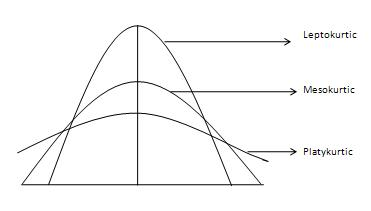
\includegraphics{curtosis.jpg}
\caption{wwwwwwwwwwwwwwww}
\end{figure}

\begin{enumerate}
\def\labelenumi{\arabic{enumi}.}
\tightlist
\item
  \textbf{Mesocurtica} : esta es la distribución normal
\item
  \textbf{Leptocurtica} : esta distribución tiene colas más gruesas y un pico más afilado. La curtosis es ``positiva'' con un valor superior a 3
\item
  \textbf{Platicurtica} : La distribución tiene un pico más bajo y más ancho y colas más delgadas. La curtosis es ``negativa'' con un valor superior a 30.263
\end{enumerate}

\begin{itemize}
\tightlist
\item
  En base a la media y desviación típica
\end{itemize}

\[k= \frac{\sum_{i=1}^{n}\left( x_i-\overline{x}\right)^4 }{ns^4};\] Si \(k=3\) además \(k\geq 3\)

\begin{itemize}
\tightlist
\item
  En base a percentiles
  \[k= \frac{P_{75}-P_{25}}{2\left( P_{90}-P_{10} \right) }\] Si \(k<3\) y si \(k=3\) ademas \(k\geq 0.263\)
\end{itemize}

Si este coeficiente es nulo, la distribución se dice normal (similar a la distribución normal de Gauss) y recibe el nombre de mesocúrtica.

Si el coeficiente es positivo, la distribución se llama leptocúrtica, más puntiaguda que la anterior. Hay una mayor concentración de los datos en torno a la media.

Si el coeficiente es negativo, la distribución se llama platicúrtica y hay una menor concentración de datos en torno a la media. sería más achatada que la primera.

\hypertarget{part-probabilidades}{%
\part{Probabilidades}\label{part-probabilidades}}

\hypertarget{experimento-aleatorio}{%
\chapter{Experimento aleatorio}\label{experimento-aleatorio}}

\begin{definition}
\protect\hypertarget{def:www}{}\label{def:www}En experimento aleatorio es un fenómeno que genera un evento
\end{definition}

\hypertarget{uxe1lgebra-de-eventos}{%
\chapter{Álgebra de eventos}\label{uxe1lgebra-de-eventos}}

Sean \(A\), \(B\) y \(C\) eventos entonces 1. e 2. wwwwwwwwwwwwwwwwwwwwwwwwwwwwww

\[ \int_{1}^{2}=\sum_{2}^{2}x_1 \]

\hypertarget{tuxe9cnicas-de-conteo}{%
\chapter{Técnicas de conteo}\label{tuxe9cnicas-de-conteo}}

\(P_n^m\) \(C_n^m\)

\[\binom{m}{n}=\frac{m}{n!(n-m)}\]

\hypertarget{definiciuxf3n-de-probabilidad}{%
\chapter{Definición de probabilidad}\label{definiciuxf3n-de-probabilidad}}

\hypertarget{probabilidad-condicional}{%
\chapter{Probabilidad condicional}\label{probabilidad-condicional}}

\leavevmode\hypertarget{wwwwwwww}{}%
wwwwwwwwwwwwwwwwww\[P(A|B)= \frac{P(B\cap A)}{P(B)}\]

\hypertarget{teorema-de-bayes}{%
\chapter{Teorema de Bayes}\label{teorema-de-bayes}}

\begin{theorem}[Teorema de Bayes]
\protect\hypertarget{thm:wwwwwwwwwwwwwwwwwwwwwwwwww}{}\label{thm:wwwwwwwwwwwwwwwwwwwwwwwwww}

Sea \(\{A_{1},A_{2},...,A_{i},...,A_{n}\}\) un conjunto de sucesos mutuamente excluyentes y exhaustivos, y tales que la probabilidad de cada uno de ellos es distinta de cero (0). Sea \(B\) un suceso cualquiera del que se conocen las probabilidades condicionales \(P(B|A_i )\). Entonces, la probabilidad \(P(A_i|B)\) viene dada por la expresión: \[P(A_i|B)=\frac{P(B|A_i)P(A_i)}{P(B)}\] donde:

\begin{enumerate}
\def\labelenumi{\arabic{enumi}.}
\tightlist
\item
  \(P(A_i)\) son las probabilidades a priori,
\item
  \(P(B|A_i)\) es la probabilidad de B en la hipótesis \(A_i\),
\item
  \(P(A_i|B)\) son las probabilidades a posteriori. :::
\end{enumerate}

\end{theorem}

\hypertarget{eventos-independientes-y-secuencias-de-experimentos}{%
\chapter{Eventos independientes y secuencias de experimentos}\label{eventos-independientes-y-secuencias-de-experimentos}}

\hypertarget{probabilidad-en-espacio}{%
\chapter{Probabilidad en espacio}\label{probabilidad-en-espacio}}

\hypertarget{part-inferencia-estaduxedstica}{%
\part{Inferencia estadística}\label{part-inferencia-estaduxedstica}}

\hypertarget{variables-aleatorias}{%
\chapter{Variables aleatorias}\label{variables-aleatorias}}

\begin{definition}[Variable aleatoria]
Sea \(\Omega\) un espacio muestral asociado a una experimento aleatorio \(\epsilon\) y \(\omega\in\Omega\), entonces se genera la función \textbf{variable aleatoria}
\begin{align*}
  X:\Omega&\longrightarrow \mathbb{R}\\
  \omega&\longmapsto X(\omega)
\end{align*}
\end{definition}

\begin{equation}
  f\left(k\right) = \binom{n}{k} p^k\left(1-p\right)^{n-k}
  \label{eq:binom}
\end{equation}

You may refer to it using \eqref{eq:binom}

\hypertarget{appendix-apendice}{%
\appendix \addcontentsline{toc}{chapter}{\appendixname}}


\hypertarget{sumatorias}{%
\chapter{Sumatorias}\label{sumatorias}}

Una suma de números representados por \(x_1, x_2, \ldots, x_n\) se simboliza en forma compacta mediante el simbolo \(\sum\) (sigma) es decir la suma de los números anteriores se puede escribir del siguiente modo \[x_1+x_2+\dots+x_n=\sum_{i=1}^nx_i.\]
Algunas propiedades son

\begin{enumerate}
\def\labelenumi{\arabic{enumi}.}
\tightlist
\item
  \(k\sum_{i=1}^nx_i=\sum_{i=1}^nkx_i\)
\item
  \(\sum_{i=1}^n\left(x_i+y_i\right)=\sum_{i=1}^nx_i+\sum_{i=1}^ny_i\)
\item
  \(\sum_{i=1}^nx_i\)
  \[\int_1^3=\lim_{n\to \infty}\sum_{i=0}^{n}f^i(x)\]
  citado por \citep{xie2015}
  Variable estadística variable estadística
\end{enumerate}

\hypertarget{ee}{%
\section{ee}\label{ee}}

\(\sum_{i=1}^nx_i\)

\[
\sum_{i=1}^n \frac{1}{2}
\]

\hypertarget{eeeee}{%
\subsection{eeeee}\label{eeeee}}

\hypertarget{matrices}{%
\chapter{Matrices}\label{matrices}}

Una matriz es un arreglo de números distribuidos en filas y columnas por ejemplo la siguiente matriz
\[A=\begin{pmatrix}
a_{11}&a_{12}&\ldots&a_{1n}\\
a_{21}&a_{22}&\ldots&a_{2n}\\
\vdots & \vdots & \ddots &\vdots \\
a_{11}&a_{11}&\ldots&a_{nm}
\end{pmatrix}_{n\times m}\]
de \textbf{orden} \(n\times m\) tiene \textbf{entradas} \(a_{ij}\) donde el primer subindice indica la fila y el segundo la columna; es usual representar por simplicidad una matriz por \(A=[a_{ij}]_{n\times m}\). Si en el orden \(n=m\) entonces la matriz recibe el nombre de \textbf{matriz cuadrada} la suma de los elementos de la diagonal de una matriz cuadrada \(\sum_{i=1}^na_{ii}\) se llama \textbf{traza}\index{traza}. Si todas las \(a_{ij}\) son cero entonces la matriz \(A=0\) recibe el nombre matriz \textbf{nula}.

Dos matrices son iguales si tienen el \textbf{mismo orden} y cada una de las entradas respectivas son iguales es decir \(A=[a_{ij}]_{n\times m}\) y \(B=[b_{ij}]_{n\times m}\) son iguales si \(a_{ij}=b_{ij}\), \(i=1,2,\ldots n\) y \(j=1,2,\ldots m\)

\hypertarget{algebra-de-matrices}{%
\section{Algebra de matrices}\label{algebra-de-matrices}}

Sean las matrices \[A=[a_{ij}]_{n\times m}=\begin{pmatrix}
a_{11}&a_{12}&\ldots&a_{1n}\\
a_{21}&a_{22}&\ldots&a_{2n}\\
\vdots & \vdots & \ddots &\vdots \\
a_{11}&a_{11}&\ldots&a_{nm}
\end{pmatrix}_{n\times m}\] y \[B=[b_{ij}]_{p\times q}=\begin{pmatrix}
b_{11}&b_{12}&\ldots&b_{1n}\\
b_{21}&b_{22}&\ldots&b_{2n}\\
\vdots & \vdots & \ddots &\vdots \\
b_{11}&b_{11}&\ldots&b_{pq}
\end{pmatrix}_{p\times q}\] entonces la suma y producto de matrices se definen

\begin{enumerate}
\def\labelenumi{\arabic{enumi}.}
\item
  Sea \(k\) un escalar entonces se verifica que \(kA=[ka_{ij}]\), \(i=1,2,\ldots n\) y \(j=1,2,\ldots m\) es decir el escalar \(k\) multiplica a cada una de las entradas de la matriz.
  \begin{align*}
  kA&=k[a_{ij}]_{n\times m}\\
  &=[ka_{ij}]_{n\times m}\\
  &=\begin{pmatrix}
  ka_{11}&ka_{12}&\ldots&ka_{1n}\\
  ka_{21}&ka_{22}&\ldots&ka_{2n}\\
  \vdots & \vdots & \ddots &\vdots \\
  ka_{11}&ka_{11}&\ldots&ka_{nm}
  \end{pmatrix}_{n\times m}
  \end{align*}
\item
  La suma o diferencia es posible si \(n=p\) y \(m=q\) es decir los ordenes de \(A\) y \(B\) son iguales, entonces la suma o diferencia resulta \begin{align*}
  A\pm B&=[a_{ij}+b_{ij}]_{n\times m}\\
  &=\begin{pmatrix}
  a_{11} + b_{11}&a_{12} + b_{12}&\ldots&a_{1n} + b_{1n}\\
  a_{21} + b_{21}&a_{22} + b_{22}&\ldots&a_{2n} + b_{2n}\\
  \vdots & \vdots & \ddots &\vdots \\
  a_{11} + b_{11}&a_{11} + b_{11}&\ldots&a_{nm} + b_{nm}
  \end{pmatrix}_{n\times m}
  \end{align*} donde \(i=1,2,\ldots n\) y \(j=1,2,\ldots m\)
\item
  El producto es posible si \(m=p\) es decir el número columnas de la primera matriz es igual al número de filas de la segunda matriz, el orden de la matriz resultante es \(n\times q\) además
  \begin{align*}
  A\cdot B&=\left[\sum_{k=1}^pa_{ik}b_{kj}\right]_{n\times q}\\
  &=\begin{pmatrix}
  \sum_{k=1}^ma_{1k}b_{k1}&\sum_{k=1}^ma_{1k}b_{k2}&\ldots&\sum_{k=1}^ma_{1k}b_{kq}\\
  \sum_{k=1}^ma_{2k}b_{k1}&\sum_{k=1}^ma_{2k}b_{k2}&\ldots&\sum_{k=1}^ma_{2k}b_{kq}\\
  \vdots & \vdots & \ddots &\vdots \\
  \sum_{k=1}^ma_{nk}b_{k1}&\sum_{k=1}^ma_{nk}b_{k2}&\ldots&\sum_{k=1}^ma_{nk}b_{kq}\\
  \end{pmatrix}_{n\times q}
  \end{align*}
\end{enumerate}

donde \(i=1,2,\ldots n\) y \(j=1,2,\ldots m\)

\begin{example}
Sean \(\begin{pmatrix} 3&-1&2\\ 2&-1&2\\ 1&-1&0\\ 5&0&0\\ \end{pmatrix}_{4\times 3}\) y \(\begin{pmatrix} 0&-1&2&2&0\\ 1&-1&-2&1&1\\ 3&-1&-3&5&2\\ \end{pmatrix}_{3\times 5}\) entonces \(A\cdot B=\begin{pmatrix} 5&-4&2&15&3\\ 5&-3&0&13&3\\ -1&0&4&1&-1\\ 0&-5&10&10&0\\ \end{pmatrix}_{4\times 5}\)
\end{example}

En caso de ser posible la multiplicación entre \(A\), \(B\) y \(C\) entonces se verfican las siguientes propiedades

\begin{enumerate}
\def\labelenumi{\arabic{enumi}.}
\tightlist
\item
  \(A(B+C)=AB+AC\)
\item
  \((A+B)C\)
\item
  \(A(BC)=(AB)C\)
\end{enumerate}

\hypertarget{matrices-particulares}{%
\section{Matrices particulares}\label{matrices-particulares}}

En esta seccion se considera las siguientes matrices: Matriz triangular, matriz particular de una matriz cuadrada,
matriz transpuesta,
matriz simetrica,
matriz conjugada,
matriz hermitica,
matriz escalonada.

\hypertarget{matriz-triangular}{%
\subsection{Matriz triangular}\label{matriz-triangular}}

Una matriz cuadrada \(A\) cuyos elementos \(a_{ij}=0\) si \(i>j\) es decir \[A=\begin{pmatrix}
a_{11}&a_{12}&\ldots&a_{1n}\\
0&a_{22}&\ldots&a_{2n}\\
\vdots & \vdots & \ddots &\vdots \\
0&0&\ldots&a_{nn}
\end{pmatrix}_{n\times n}\] se llama \textbf{matriz triangular superior}; reciprocamente si \(i<j\) es decir \[A=\begin{pmatrix}
a_{11}&0&\ldots&0\\
a_{21}&a_{22}&\ldots&0\\
\vdots & \vdots & \ddots &\vdots \\
a_{11}&a_{11}&\ldots&a_{nn}
\end{pmatrix}_{n\times n}\] se llama \textbf{matriz triangular inferior}. Si \(A\) es a la vez \textbf{matriz triangular superior} y \textbf{matriz triangular inferior} entonces recibe el nombre de \textbf{matriz diagonal}, representada por
\[
\left(a_{11}, a_{22}, \ldots, a_{nn}\right)
\]
además si \(a_{11}= a_{22}= \ldots = a_{nn}=k\) la matriz recibe el nombre de \textbf{matriz escalar} y si \(k=1\) la matriz recibe el nombre de \textbf{matriz unidad} representada por \(I_n\) por ejemplo
\[I_3=\begin{pmatrix}
1  & 0 & 0 \\
0  & 1 & 0 \\
0  & 0 & 1 \\
\end{pmatrix}
\]

\hypertarget{matriz-particular-de-una-matriz-cuadrada}{%
\subsection{Matriz particular de una matriz cuadrada}\label{matriz-particular-de-una-matriz-cuadrada}}

\hypertarget{matriz-transpuesta}{%
\subsection{Matriz transpuesta}\label{matriz-transpuesta}}

\hypertarget{matriz-simetrica}{%
\subsection{Matriz simetrica}\label{matriz-simetrica}}

\hypertarget{matriz-conjugada}{%
\subsection{Matriz conjugada}\label{matriz-conjugada}}

\hypertarget{matriz-hermitica}{%
\subsection{Matriz hermitica}\label{matriz-hermitica}}

\hypertarget{matriz-escalonada}{%
\subsection{Matriz escalonada}\label{matriz-escalonada}}

\[
\begin{pmatrix}
 w & warnwww   & w \\
 w & warnwww   & w \\
\end{pmatrix}_{4\times 3}
\]

\begin{Shaded}
\begin{Highlighting}[]
\NormalTok{xw }\OtherTok{=} \StringTok{\textquotesingle{}Es decir los elementos son demagogos y déspotas\textquotesingle{}}
\NormalTok{x1 }\OtherTok{=} \StringTok{\textquotesingle{}Es decir los elementos son demagogos y déspotas\textquotesingle{}}
\end{Highlighting}
\end{Shaded}

\[
\frac{\sin x}{x^3}
= 0.3794281
\]

\[
\Phi_{\mu , \sigma ^{2}}(x)=\frac {1}{\sigma {\sqrt {2\pi }}}e^{-{\frac {(u-\mu )^{2}}{2\sigma ^{2}}}}du
\]

\begin{enumerate}
\def\labelenumi{\arabic{enumi}.}
\item
  Www \[\frac{1}{20\sqrt{2\pi }}\int_{-\infty }^{ 300}e^{- \frac{1}{2}\left(\frac{z-200}{20}\right)^2}dz=0.9999997\]
\item
  0.9500042 also Es decir los elementos son demagogos y déspotas
\item
  Es decir los elementos son demagogos y déspotas
\end{enumerate}

Tabla \ref{tab:ww1}

\begin{longtable}[]{@{}
  >{\raggedleft\arraybackslash}p{(\columnwidth - 8\tabcolsep) * \real{0.11}}
  >{\centering\arraybackslash}p{(\columnwidth - 8\tabcolsep) * \real{0.04}}
  >{\raggedright\arraybackslash}p{(\columnwidth - 8\tabcolsep) * \real{0.02}}
  >{\raggedleft\arraybackslash}p{(\columnwidth - 8\tabcolsep) * \real{0.25}}
  >{\raggedright\arraybackslash}p{(\columnwidth - 8\tabcolsep) * \real{0.57}}@{}}
\caption{\label{tab:ww1} Caption}\tabularnewline
\toprule
Option & N & w & Observation & Description \\
\midrule
\endfirsthead
\toprule
Option & N & w & Observation & Description \\
\midrule
\endhead
Es decir los elementos son demagogos y déspotas Es decir los elementos son demagogos y déspotas & 1 & w & Es decir los elementos son demagogos y déspotas & Es decir los elementos son demagogos y déspotas Es decir los elementos son demagogos y déspotas \\
Engine & 2 & w & Es decir los elementos son demagogos y déspotas \(\sum^{n}_{i=1}{f_i}\) & Engine to be used for processing templates. Handlebars is the default. \\
Es decir los elementos son demagogos y déspotas & 3 & w & \(\sum^{n}_{i=1}{f_i}\) & extension to be used for dest files. \\
\bottomrule
\end{longtable}

variable aleatoria Variable aleatoria entonces

2.7182818 0.9750021 0.7881446

2561

The value of \texttt{x} in the Python session is Es decir los elementos son demagogos y déspotas .
It is not the same \texttt{x} as the one in R.

\begin{figure}

{\centering 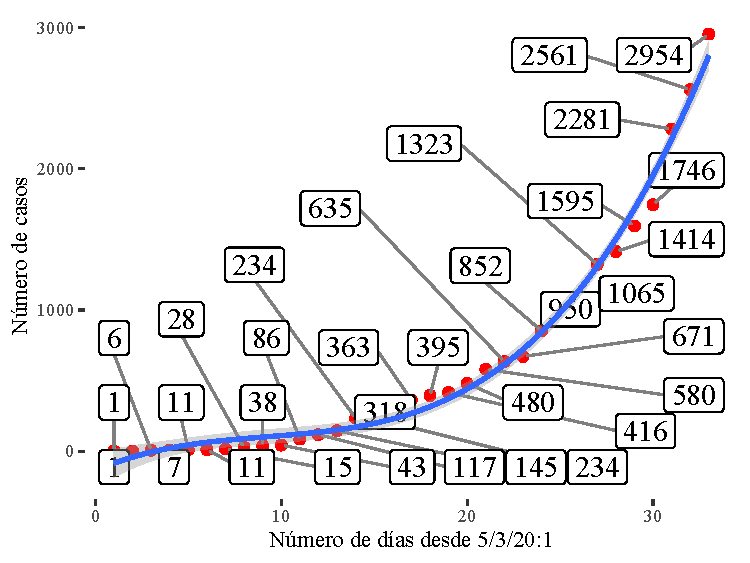
\includegraphics{E_1_files/figure-latex/ww1w-1} 

}

\caption{Regresión lineal}\label{fig:ww1w}
\end{figure}

\begin{verbatim}
## (Intercept) 
##    12917.13
\end{verbatim}

  \bibliography{book.bib,packages.bib}

\printindex

\end{document}
